%!TEX program = xelatex
% 完整编译: xelatex -> bibtex -> xelatex -> xelatex
\documentclass[lang=cn,11pt,a4paper,cite=authoryear]{elegantpaper}

\title{电商用户商品价值评估及基于图神经网络的个性化推荐系统}
\author{徐璨 \and 章寅 \and 钱少璐}
\institute{浙江工商大学}

% \version{0.09}
\date{}


% 本文档命令
\usepackage{array}
%for long table
\usepackage{longtable}
% \usepackage{arydshln}
\usepackage{float}
\usepackage{graphicx}
\newcommand{\ccr}[1]{\makecell{{\color{#1}\rule{1cm}{1cm}}}}
\newcommand{\PreserveBackslash}[1]{\let\temp=\\#1\let\\=\temp}
\newcolumntype{C}[1]{>{\PreserveBackslash\centering}p{#1}}
\newcolumntype{R}[1]{>{\PreserveBackslash\raggedleft}p{#1}}
\newcolumntype{L}[1]{>{\PreserveBackslash\raggedright}p{#1}}
\begin{document}

\maketitle

\begin{abstract}
  对商品价值和用户价值的分析在如今大数据时代能够帮助电商平台和商家指定有效的营销手段以提升其商业表现,且随着有关推荐系统研究的发展,平台能够根据历史交易数据对用户进行个性化推荐以提升用户的转化率,进而提升企业营业水平。本文为了商品和用户的价值评估,分别提取了基于商品和基于用户的一系列特征。对于商品的价值评估,本文对获得的特征进行主成分分析降维,并运用K-Means++和DBSCAN聚类算法探索对商品进行有效分类。最终运用5分类的K-Means++聚类算法得到了能够有效反映商品畅销程度,盈利水平,退货率高低等特征的商品分类。对于用户价值评估,本文采用改进RFM模型,采用中位数作为划分阈值,对用户实现价值划分。随后本文介绍了贝叶斯个性化排序推荐(BPR),和基于图神经网络(GNN)的图神经网络协同过滤(NGCF)和轻量化图卷积网络(LGCN)模型。并于此基础上,创新性的提出了宽图卷积网络(WideGCN)以实现对商品,用户特征的有效利用。本文提出的WideGCN在多项推荐系统评价指标上都稳定优于目前最新,最流行的推荐系统算法。
\keywords{K-Means++聚类,RFM模型,GNN,BPR,LGCN,WideGCN}
\end{abstract}


\section{引言}
如今高度成熟的互联网经济不仅显著改变了人们的生活方式,也促进了相关行业的发展。通过有效运用互联网中的人和物生成海量数据,企业能够显著提升其营业水平。从商家角度而言,对于商品数据的有效分析能够帮助商家优化库存,提升营销效果,对于用户数据的有效分析则能为商家针对性采取措施提供依据,帮助提升用户的转化率,复购率等从而帮助商家提升经营水平。除了针对商品和用户数据进行数据挖掘外,利用其进行推荐系统模型构建也是企业提升营业水平和用户使用体验一个研究方向。从本世纪初至今,诸多经营电商,文娱业务互联网公司通过推荐系统模型针对不同用户进行个性化推荐,极大的提升了其企业商业表现的同时,也提升了用户在购物,娱乐等方面的体验。

在电商场景中,随着商品数量的爆炸性增长,用户在选购商品时面对成千上万的搜索结果可能难以做出决定,因此,个性化的推荐能够生成满足用户需求和喜爱的商品排序表,从而提升用户选购体验的同时帮助商家提升营业水平。

本文的主要工作可以总结为以下几点:

\begin{itemize}
  \item [(1)] 
  对数据进行预处理,提取出基于商品和用户的特征
  \item [(2)]
  对提取到的商品特征进行主成分分析,并综合尝试K-Means++和DBSCAN算法构建商品分类模型,并实现商品在畅销程度、盈利能力和退货水平等维度上的有效划分。
  \item [(3)]
  基于RFM模型理论,结合本文提取到的用户特征,对RFM模型中的指标进行新的改进,并有效划分出8类用户群体,实现对高价值用户等用户群的有效划分。
  \item[(4)]
  利用基于图神经网络的推荐系统模型,构建BPR,NGCF,LGCN模型实现对用户的个性化排序推荐。
  \item[(5)]
  综合考虑上文提取的基于商品和用户的特征,结合LGCN模型的思想,创新性地提出WideGCN思想,利用商品用户特征这类旁系特征实现更好地个性化排序推荐效果。 
\end{itemize}

\section{数据预处理}

本文训练集源于某礼品批发平台于2010年12月1日至2011年11月30日内的订单信息,共有389169条商品交易信息。主要信息包括发票号码,产品代码,产品描述,单笔产品交易数量,订单日期,商品单价,顾客代码及所在国家。总计389169条信息中,有1848条为非产品信息,例如邮费,手工退费,银行收费等。所有信息中,订单数共计21269个,产品共计3676种,其中8种非产品,顾客人数共计4331人,一年内平台实际成交额为7957559.434英镑。

\subsection{基于商品的特征工程}

训练集中的产品-用户交互信息无法直接用于判别产品的价值,故特征提取是分析商品价值的一个重要部分。故要分析商品的畅销程度,盈利能力和退货率等需要构建基于商品的一系列特征。为了分析商品的商业价值,本文从商品订单单数,销量,销售额,购买者数量,复购次数,下单间隔,退货率等角度提取了相关特征。具体提取的特征如\tabref{基于商品的特征}所示:

\begin{table}[!htb]
  \centering
  \caption{基于商品的特征}
    \huge
    \begin{tabular}{c|c}
    \hline
    \textbf{特征名称} & \textbf{备注} \\
    \hline
    total orders  & 总下单量 \\
    total sales    & 总销售量 \\
    maximum/minimum/mean/median sales & 每单最大/最小/平均/中位销量  \\
    sales figure   & 总销售额 \\
    maximum/minimum/mean/median figure & 每单最大/最小/平均/中位销售额 \\
    customer count & 下单客户人数 \\
    maxinmum/mean order per customer & 最大/平均复购次数 \\
    return ratio & 退货率 \\
    maximum order gap & 最长下单间隔 \\
    \hline
    \end{tabular}
  \label{基于商品的特征}
\end{table}

针对商品价值评估,本文认为订单数,销量,购买者人数,复购次数和下单间隔能够很好的反应商品的畅销程度。越畅销的商品,其订单数,销量,购买人数,复购次数越大,下单间隔越短。至于商品的盈利能力,本文在缺少商品成本信息的情况下,选取销售额,购买者次数,复购次数等作为评价指标。而商品情况可以直接通过退货率来表现。

初步分析提取出的商品信息,订单数超过1000的有14款商品,销量超过20000的有13款商品,有38件商品在超过30天内未被下单,另外也有部分商品存在100\%或者超高退回率的情况。

\figref{商品特征相关性矩阵}为本文提取的基于商品的特征相关性矩阵,可以见得本文提取的特征之间相关系数适中,较好的避免了特征的强相关性,故特征不存在冗余,同时一定程度相关的特征也为后续的主成分分析提供了先决条件。
\begin{figure}[H]
  \centering
  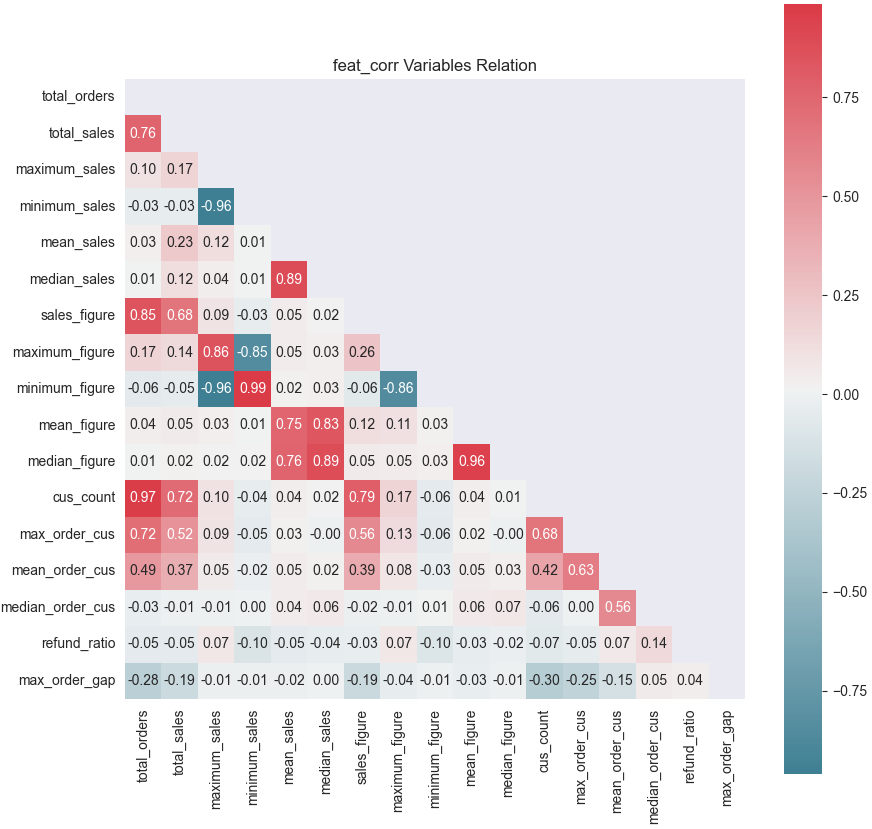
\includegraphics[width=12cm]{feat_corr.png}
  \caption{商品特征相关性矩阵}
  \label{商品特征相关性矩阵}
\end{figure}

\subsection{基于用户的特征工程}
与基于商品的特征工程类似,本文为了分析用户对平台的价值,根据RFM模型相关理论提取了一系列基于用户的特征。包括一年内用户下单次数,购买商品数量,购买金额,退货率及有效订单的平均金额等指标。具体提取的特征如\ref{基于用户的特征}所示:
\begin{center}
\begin{longtable}{c|c}
    \caption{基于用户的特征}
    \label{基于用户的特征}\\
    \hline
      \textbf{特征名称} & \textbf{备注} \\
      \hline
      user total orders  & 下单量 \\
      user total purchase  & 总购买商品量 \\
      maximum/minimum/mean/median purchase figure & 每单最大/最小/平均/中位购买金额  \\
      total purchase figure   & 总购买金额 \\
      return ratio & 退货率 \\
      return figure ratio & 退款率 \\
      mean valid purchase figure & 平均有效订单金额 \\
      recent purchase gap & 最近一次消费距2011-11-30天数间隔 \\
      maximum purchase gap & 最初最终消费间隔 \\
      purchase type & 购买商品种类 \\
      maximum/minimum/mean purchase  & 最大/最小/平均购买种类 \\
      \hline
  \end{longtable}
\end{center}

本文在提取出的以上信息包括了4331余名用户的16个特征,提取上述特征的数量显然超过了本文接下来用于用户价值分类的RFM模型所需。提取16个特征更多的是服务于后文中提出的创新性的WideGCN模型。\figref{客户下单情况分布}中做出了用户下单次数和下单金额在各区间内的人数分布情况。可见该电商平台的用户粘性还是较大,大部分客户在一年间下单次数集中在10至300次区间。相应的,众多客户下金额集中在10至2000英镑区间内。
\begin{figure}[H]
  \centering
  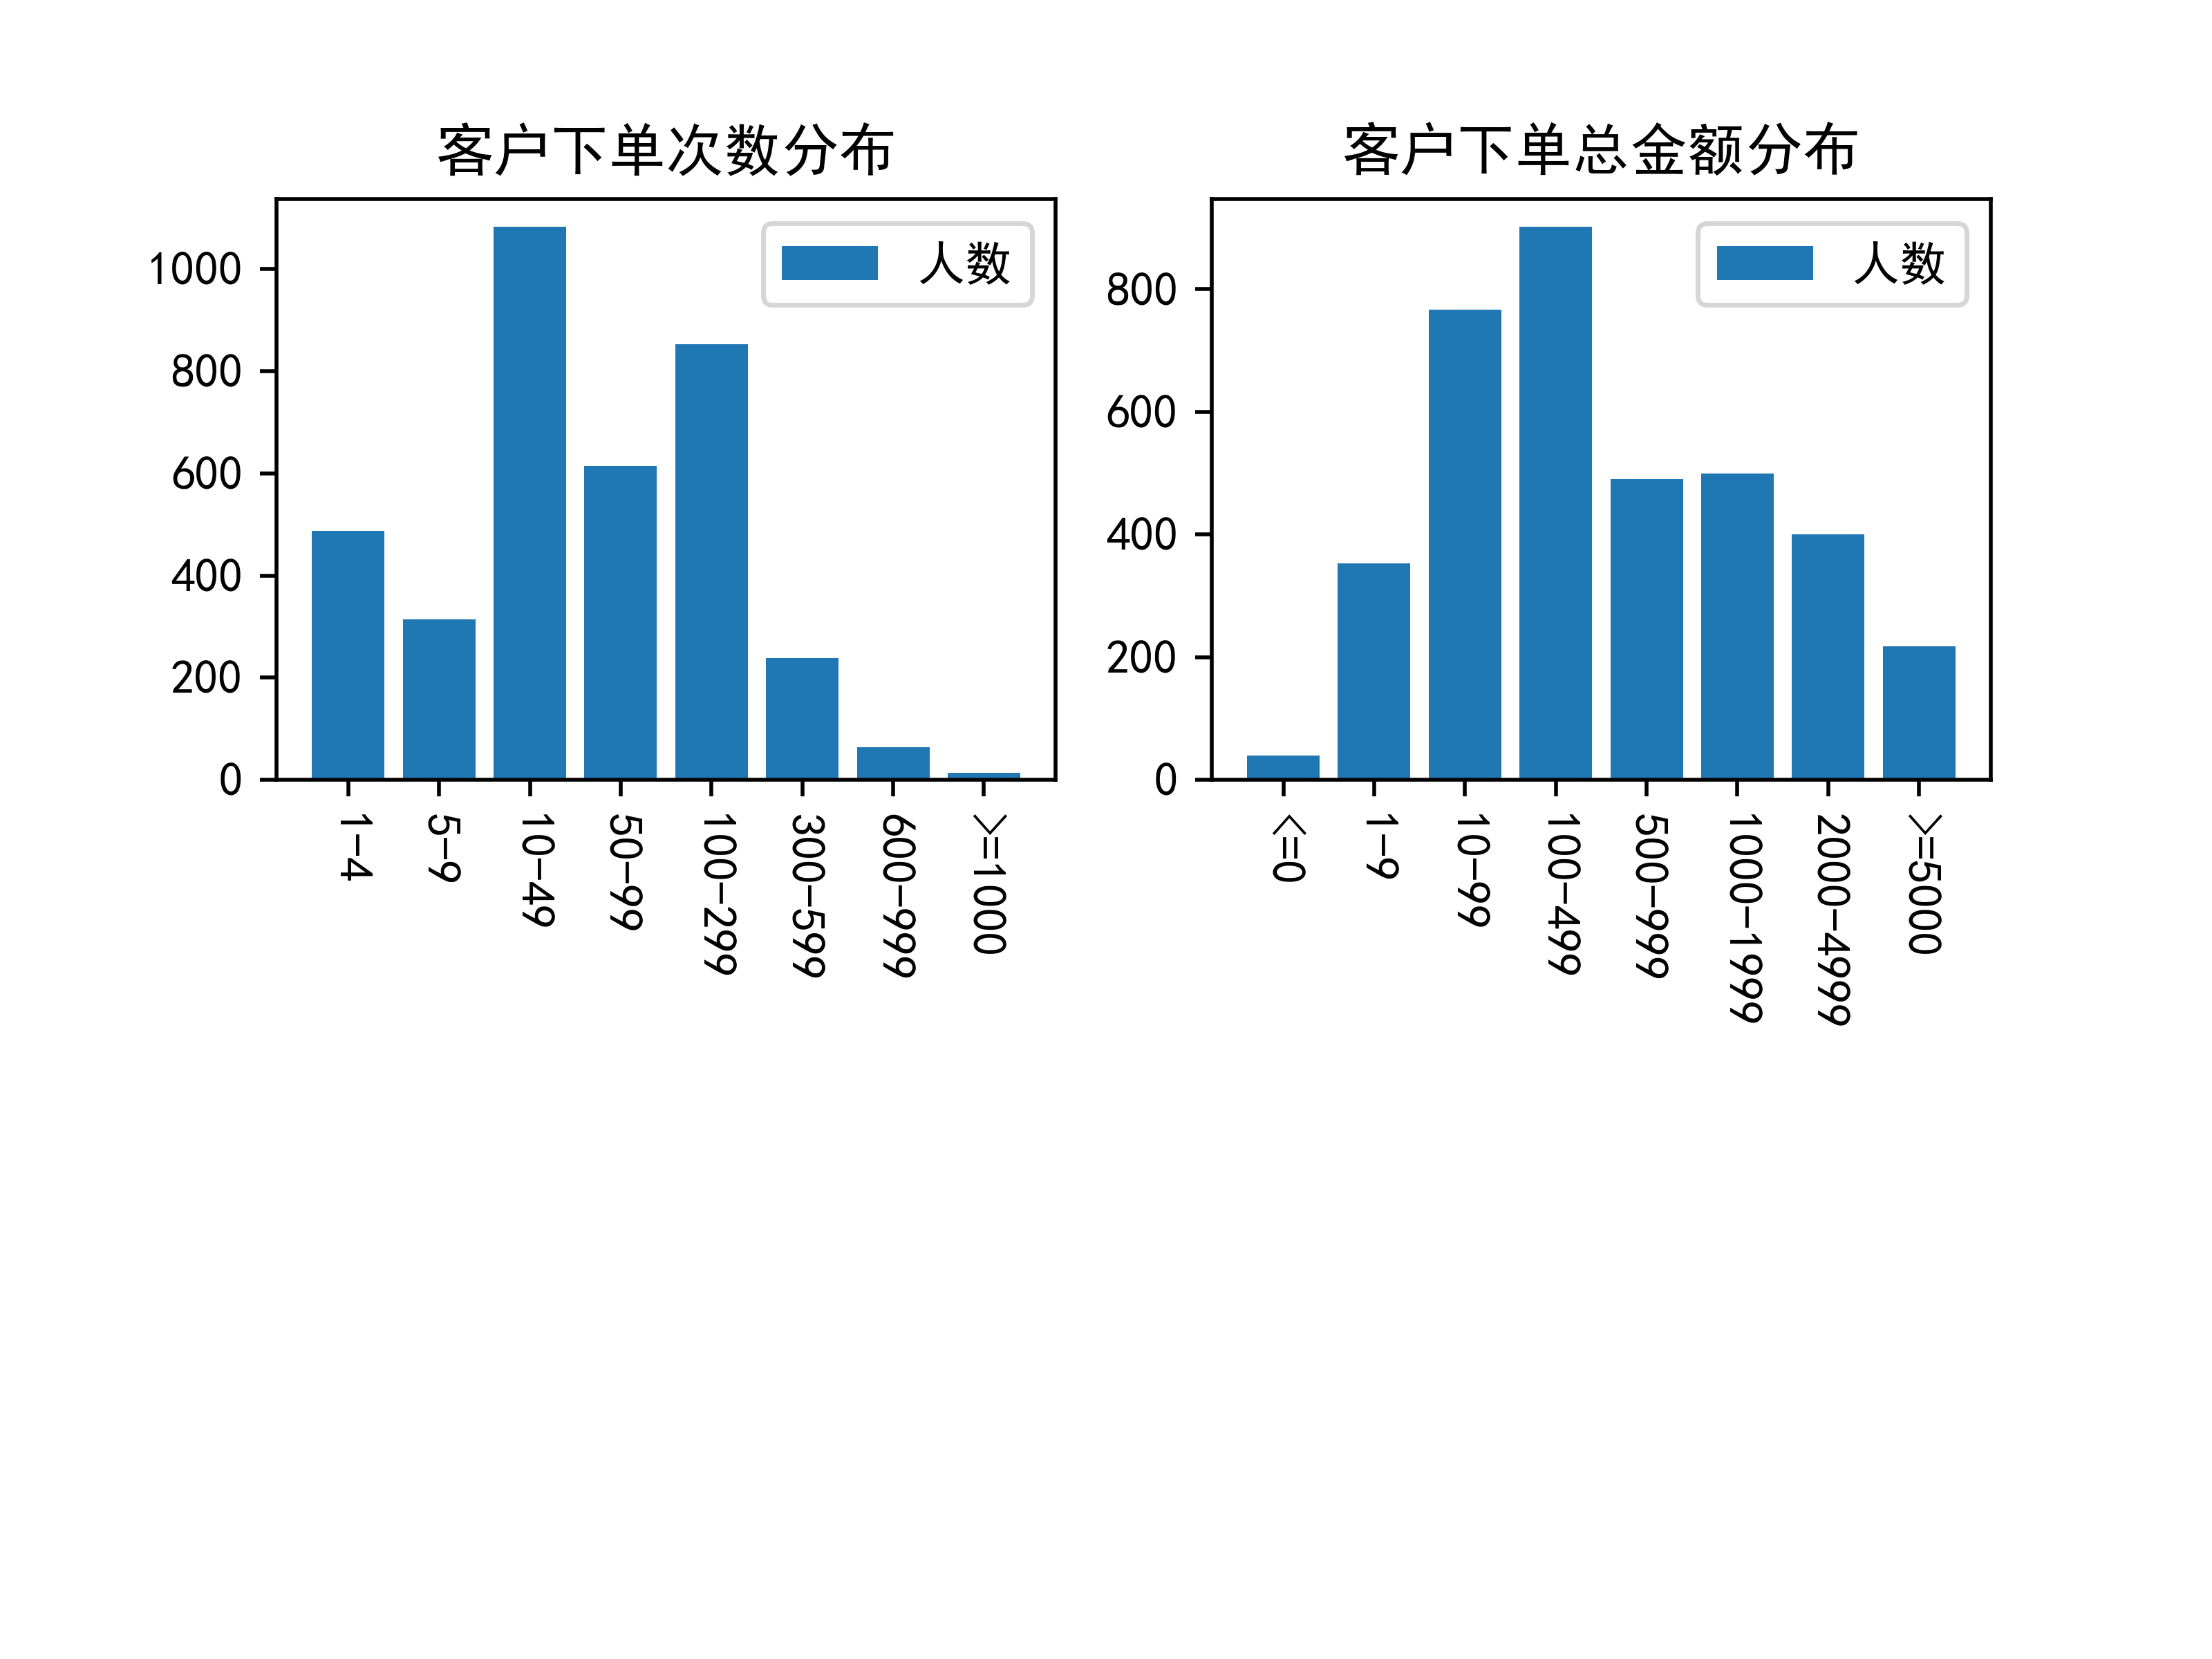
\includegraphics[width=12cm]{user_orders.png}
  \caption{客户下单情况分布}
  \label{客户下单情况分布}
\end{figure}

\section{平台商品价值分析}

\subsection{特征降维}

在基于商品的特征工程中,本文提取了16个特征,涵盖商品的销量,覆盖人群,购买频率,退货率等多个方面。为简化变量结构,本文将首先对变量进行主成分分析(PCA),在此之前,本文先对模型进行了标准化。

主成分分析的目标就是将高维随机变量映射至低维随机变量空间内,并希望保留尽可能多的信息。$X_{m \times n}$表示经过标准化后的$m$个$n$维数据的矩阵,其协方差矩阵为$\Sigma$,对其做特征值分解。考虑将$m$维随机变量$X_{m \times n}$映射到随机变量$Y$的线性变换:

\begin{equation}
  y_i = \alpha_{i}^T X = \alpha_{1i}x_1 +\alpha_{2i} x_2 + \cdots + \alpha_{mi} x_m
\end{equation}

其中$\alpha_i^T = (\alpha_{1i}, \alpha_{2i}, \cdots, \alpha_{mi})$为协方差矩阵的特征向量矩阵。要运用主成分分析,首先需要对上文提取的基于商品的特征进行标准化,以去除不同特征间量纲的差异。其次需要对数据进行适用性检验,即要分析变量之间的相关性。根据\figref{商品特征相关性矩阵}可见,大多数简单相关系数大小适中,同时采取了KMO(Kaiser-Meyer-Olkin)检验用于比较特征间的简单相关系数和偏自相关系数的相对大小。根据检验结果,本文选取的特征的KMO检验统计量为0.7,认为原始数据中存在公共因子。

为了在较少的信息损失的前提下,将高维数据转换为低维数据,本文运用主成分分析的方法。\figref{主成分聚类}中的左子图表示各主成分解释方差的占比和累计方差占比,其中前三个主成分的解释方差累计占比达87\%,故本文选取3个主成分用于后续建模。
\begin{figure}[H]
  \centering
  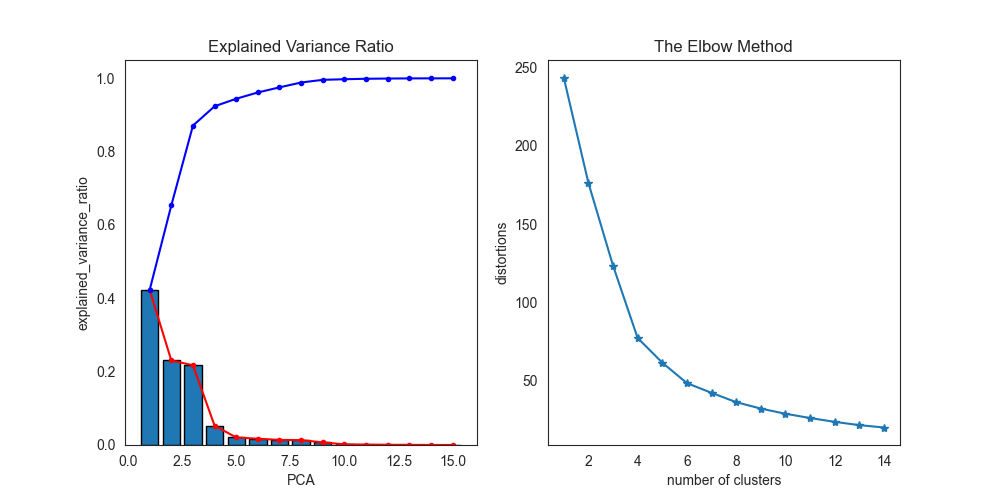
\includegraphics[width=\textwidth]{pca-kmeans-em.png}
  \caption{PCA解释方差占比图及Kmeans聚类$k-SSE$关系图}
  \label{主成分聚类}
\end{figure}

随后\figref{因子载荷矩阵}给出三个主成分的因子载荷矩阵。
\begin{figure}[H]
  \centering
  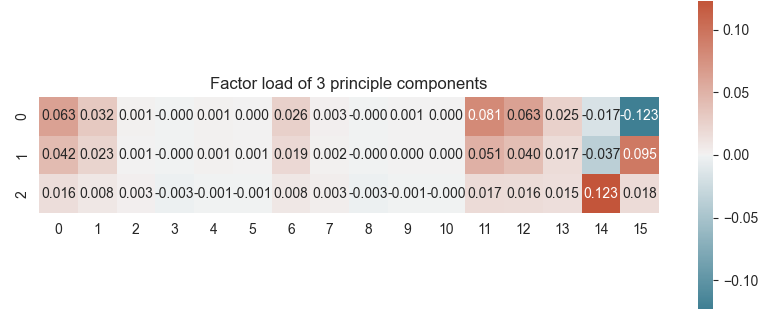
\includegraphics[width=\textwidth]{factor-load.png}
  \caption{解释方差占比前三主成分的因子载荷矩阵}
  \label{因子载荷矩阵}
\end{figure}

从\figref{因子载荷矩阵}中可以见得,解释方差占比最大的主成分受订单数,销量和覆盖客户率的影响相对更大,解释方差占比第三的主成分受退货率影响相对更大。经过上述操作,本文成功的将16维特征数据降到3维,在保证信息损失较小的情况下,为下述聚类分析奠定基础。

\subsection{聚类分析}

聚类分析是一种根据样本的观测特征,通过特定方法,将样本实施分类的方法。通过此法,能通过研究分类的特征代替研究具体样本的特征,减少研究对象的数目。在有效的聚类分析下,一个分类中的研究对象的特征在某些方面具备较大相似性,不同分类的研究对象彼此间具有明显的差异性。从机器学习的角度来讲,不同于分类问题,聚类分析是一种无监督学习,因为预先无法获悉观测样本的分类。为了分析商品在畅销性、盈利能力和退货率等维度下的分类,本文选取了两种能够处理连续性样本特征的聚类分析方法:K-Means++和DBSCAN。

K-Means算法是一种常见的聚类算法,其会将研究对象划分为$k$个簇。其首先会选取$k$个点作为初始质心,通过计算每个样本到各质心的欧氏距离,将样本分入距离最近的质心所在簇,通过计算簇内样本特征的均值,并使用均值作为该簇新的质心,随后重复计算每个样本到质心的欧氏距离,直至模型收敛或达到最大迭代次数。但此法在实际应用中存在受初始质心影响较大,容易产生空簇和局部收敛的劣势,故本文选取基于K-Means的改进K-Means++算法进行聚类分析。两者差异在于K-Means++初始只选择一个点作为质心,通过计算每个样本到该质心的欧氏距离,选择距离当前质心最远的点作为下一个质心,重复知道选择出$k$质心。此方法能够很好降低算法受初始质心选择的影响。

上述聚类算法是基于欧氏距离的,而有时候数据是非球状时,基于距离的聚类算法效果可能不佳。DBSCAN算法是基于密度对样本实施聚类的算法,通过寻找被低密度区域分隔开的高密度区域,能够将任意形状的高密度区域划分为独立类别。DBSCAN(Density-Based Spatial Clustering of Application with Noise,具有噪声的基于密度的聚类方法)中的簇不再是距离相近的点的集合,而是密度相连的点的最大集合。在DBSCAN算法中,数据被分为了三类:核心点,边界点和噪音点。核心点指以$eps$为半径的邻域至少包含了$MinPts$个样本的样本,边界点指在其他核心点邻域内但自身邻域样本数目小于$MinPts$的样本,此外既非核心点又非边界点的则是噪音点。

在聚类过程中,首先任选一样本点,找到与这个样本点距离小于等于$eps$的所有点,如果起始点$eps$半径内的数据点小于$MinPts$则被标记为噪音点,若大于$MinPts$则被标记为核心点,分为一个簇。随后访问该点以$eps$为半径的邻域内的点,并分配到该簇内,若邻域内的点也是核心点,就重复该步骤,直到该簇不再有新的核心点加入。随后访问尚未被访问的点,重复上述步骤即可。

\subsection{模型构建}

在此部分,本文将对经过主成分分析降维后的商品特征数据进行聚类,用以分析该电商平台商品在畅销程度、盈利能力和退货率等层面的表现。

本文首先基于K-Means++算法构建聚类模型。在K-Means++算法中,$k$值的选择是至关重要的,本文将基于手肘法和轮廓系数评估合适的$k$值取值。手肘法即计算不同$k$值取值时模型的误差平方和(SSE),随着$k$值增大,SSE也会随之下降,在$k$值较小时,SSE的下降幅度较大,而$k$值变大时,聚合程度提高在SSE层面带来的回报会骤减。因此一般认为SSE随$k$值增大而下降趋势变缓的临界点取值为合适的$k$的取值,\figref{主成分聚类}的右子图为本文输出的$k$-SSE关系图.

依据上述理论,$k$的理想取值应当为4。在$k \geqslant 5$的情况下,SSE的下降率有所减缓。通过手肘法选取$k$值比较直观,但比较粗糙,使用平均轮廓系数(Average Silhouette Coefficient)能够帮助更加精确选择$k$值。

\begin{equation}
  S(i) = \frac{b(i)-a(i)}{max \{a(i), b(i) \}}
\end{equation}

对于一个样本点$i$,其中$a(i)$表示簇中所有点到其距离均值,$b(i)$表示$i$到其他簇内点距离均值的最小值。其取值介于$[-1, 1]$。簇内样本点距离越小,簇间样本点距离越大,则平均轮廓系数越大$S(i)$,即代表聚类效果越好。\tabref{平均轮廓系数表}表示了在$k$取2到8时平均轮廓系数的大小。
\begin{table}[!htb]
  \centering
  \caption{样本平均轮廓系数表}
    \huge
    \begin{tabular}{c|c}
    \hline
    \textbf{$k$} & \textbf{平均轮廓系数} \\
    \hline
    2 & 0.42510056068707935 \\
    3 & 0.46681957837945537 \\
    4 & 0.49967257239768886 \\
    5 & 0.43386757407468374 \\
    6 & 0.42604697736033786 \\
    7 & 0.3897748768407509  \\
    8 & 0.39884295665316416 \\
    \hline
    \end{tabular}
  \label{平均轮廓系数表}
\end{table}

\tabref{平均轮廓系数表}中显示出当$k$取3,4,5时平均轮廓系数较大,其中$k$取4时聚类效果最优。\figref{平均轮廓系数}为$k$取4和5时轮廓系数图。
\begin{figure}[H]
  \centering
  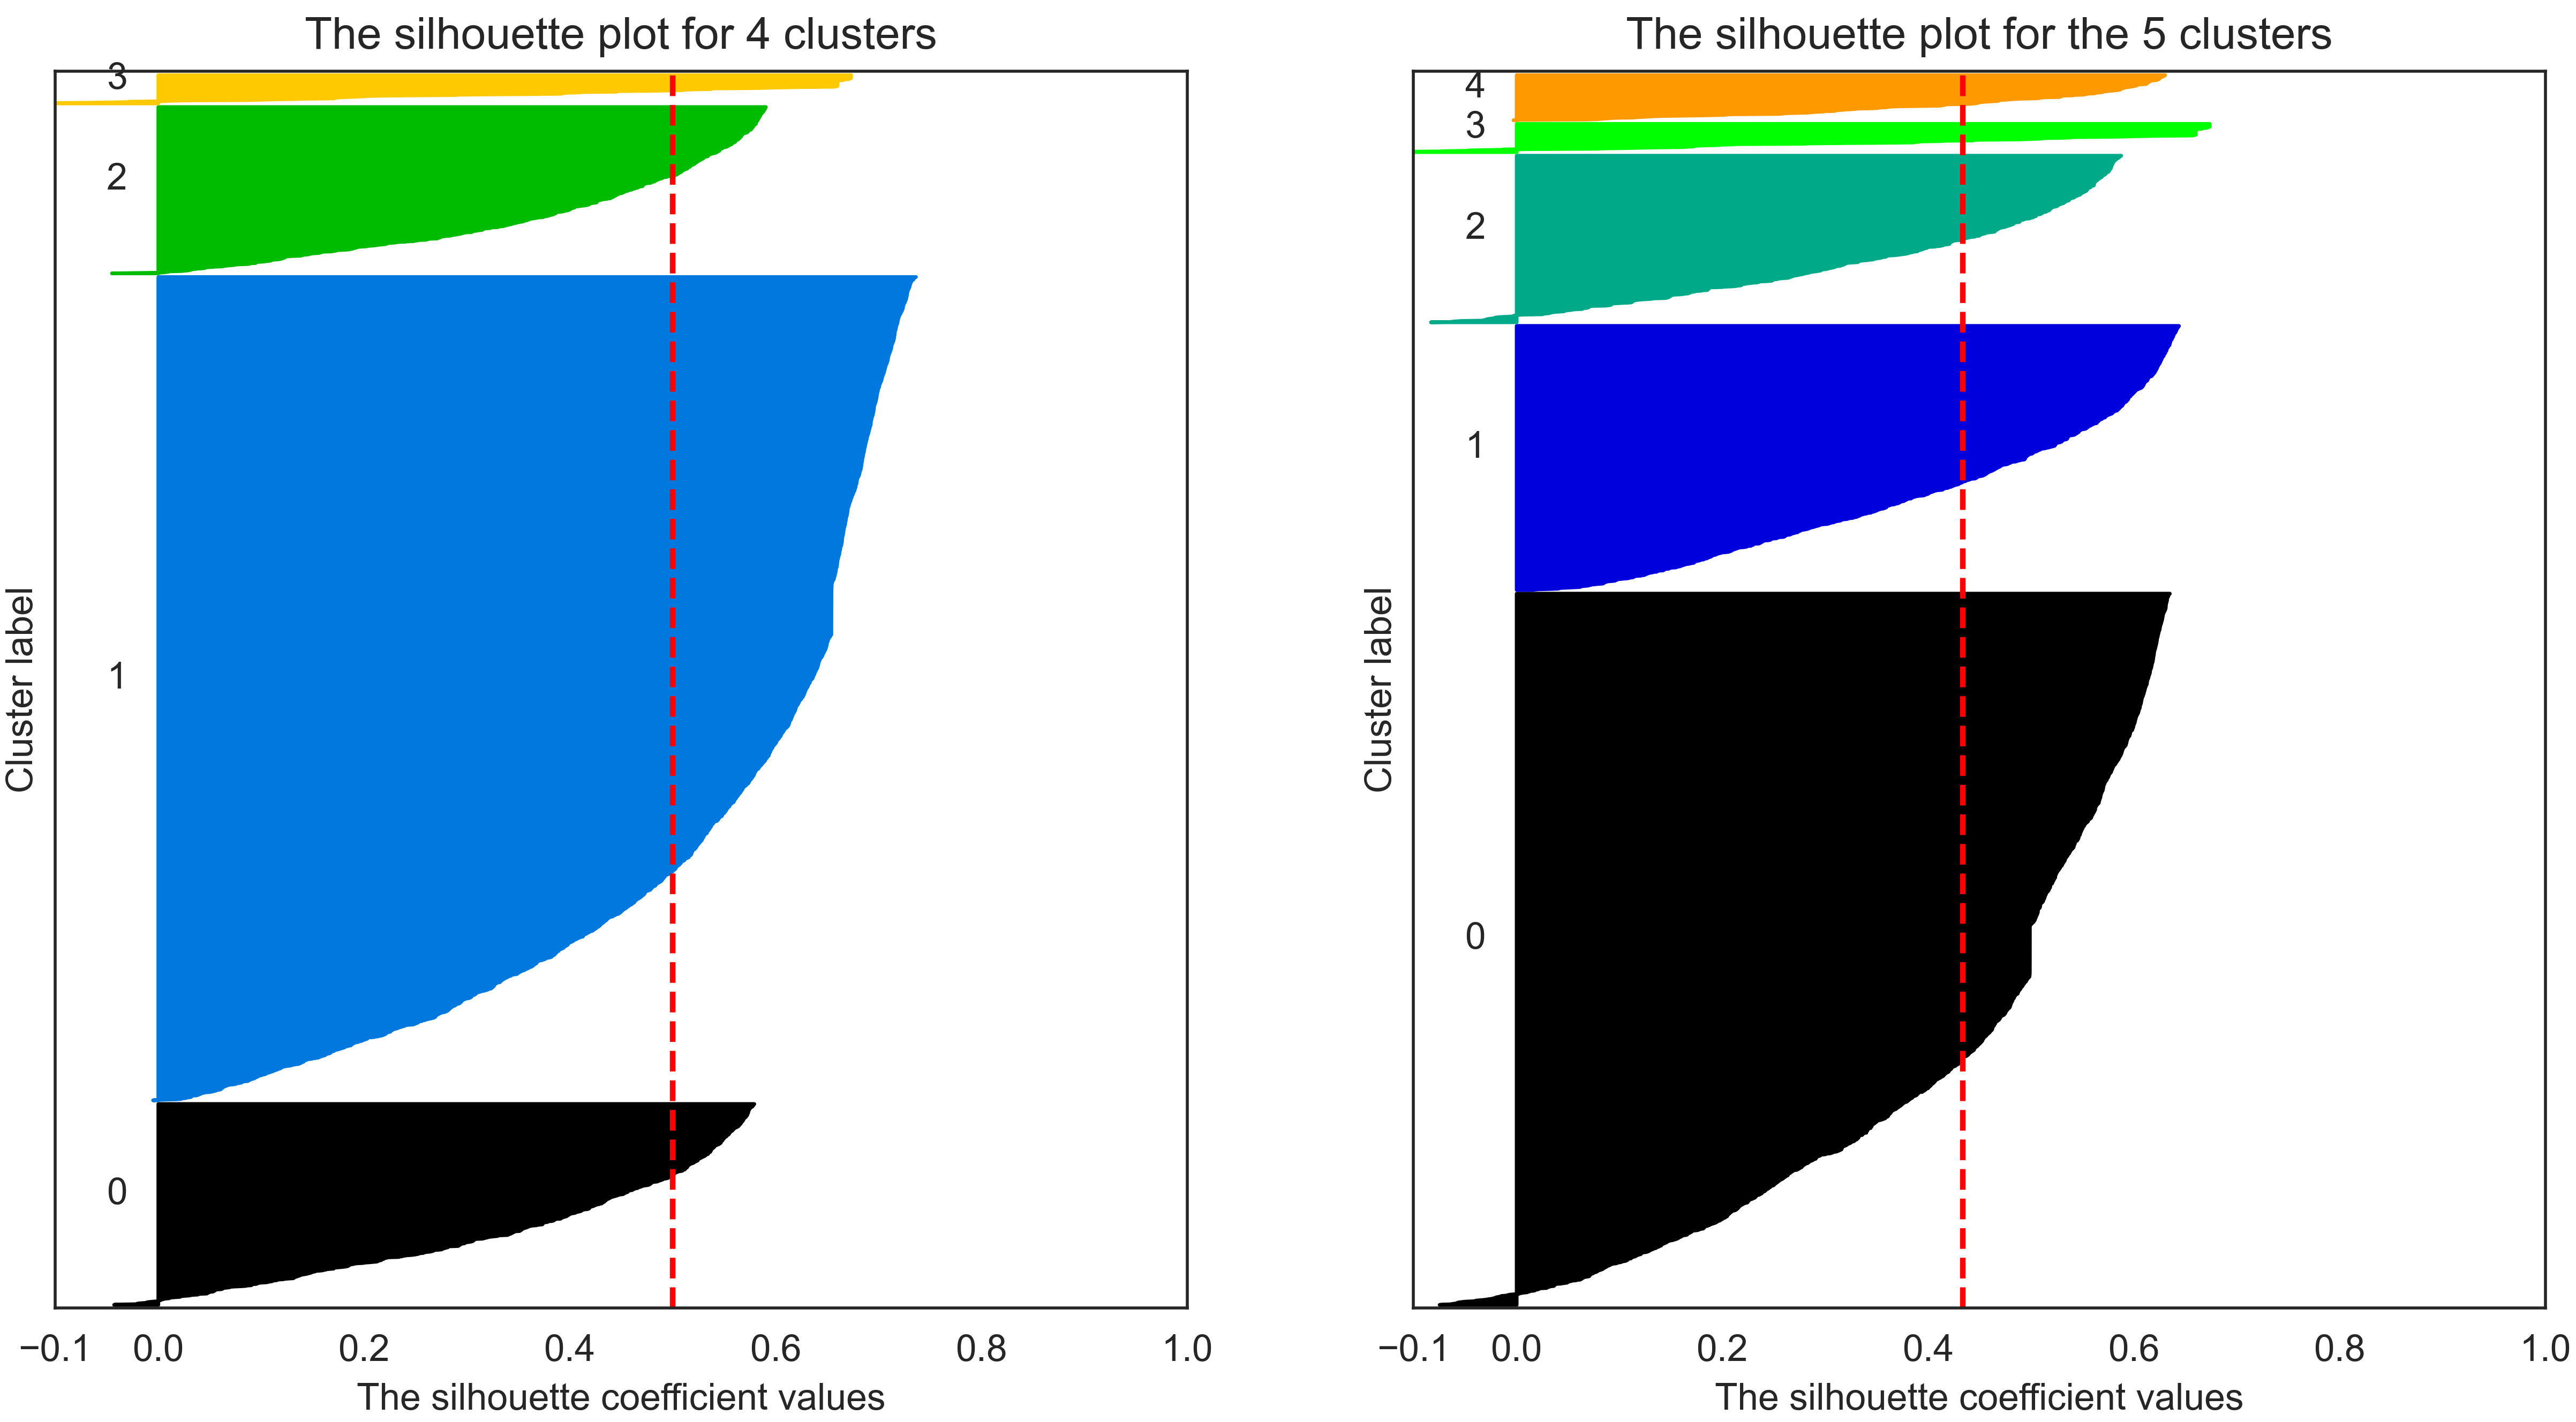
\includegraphics[width=\textwidth]{silhouette-45.png}
  \caption{解释方差占比前三主成分的因子载荷矩阵}
  \label{平均轮廓系数}
\end{figure}

根据上述分析,本文选择$k$取值为4的K-Means++算法对所有三千余件商品进行聚类操作。\figref{4聚类二维三维图}表示了$k=4$时样本点于前两个主成分构成二维空间的投影图和于三个主成分构成的三维空间的投影图。
\begin{figure}[H]
  \centering
  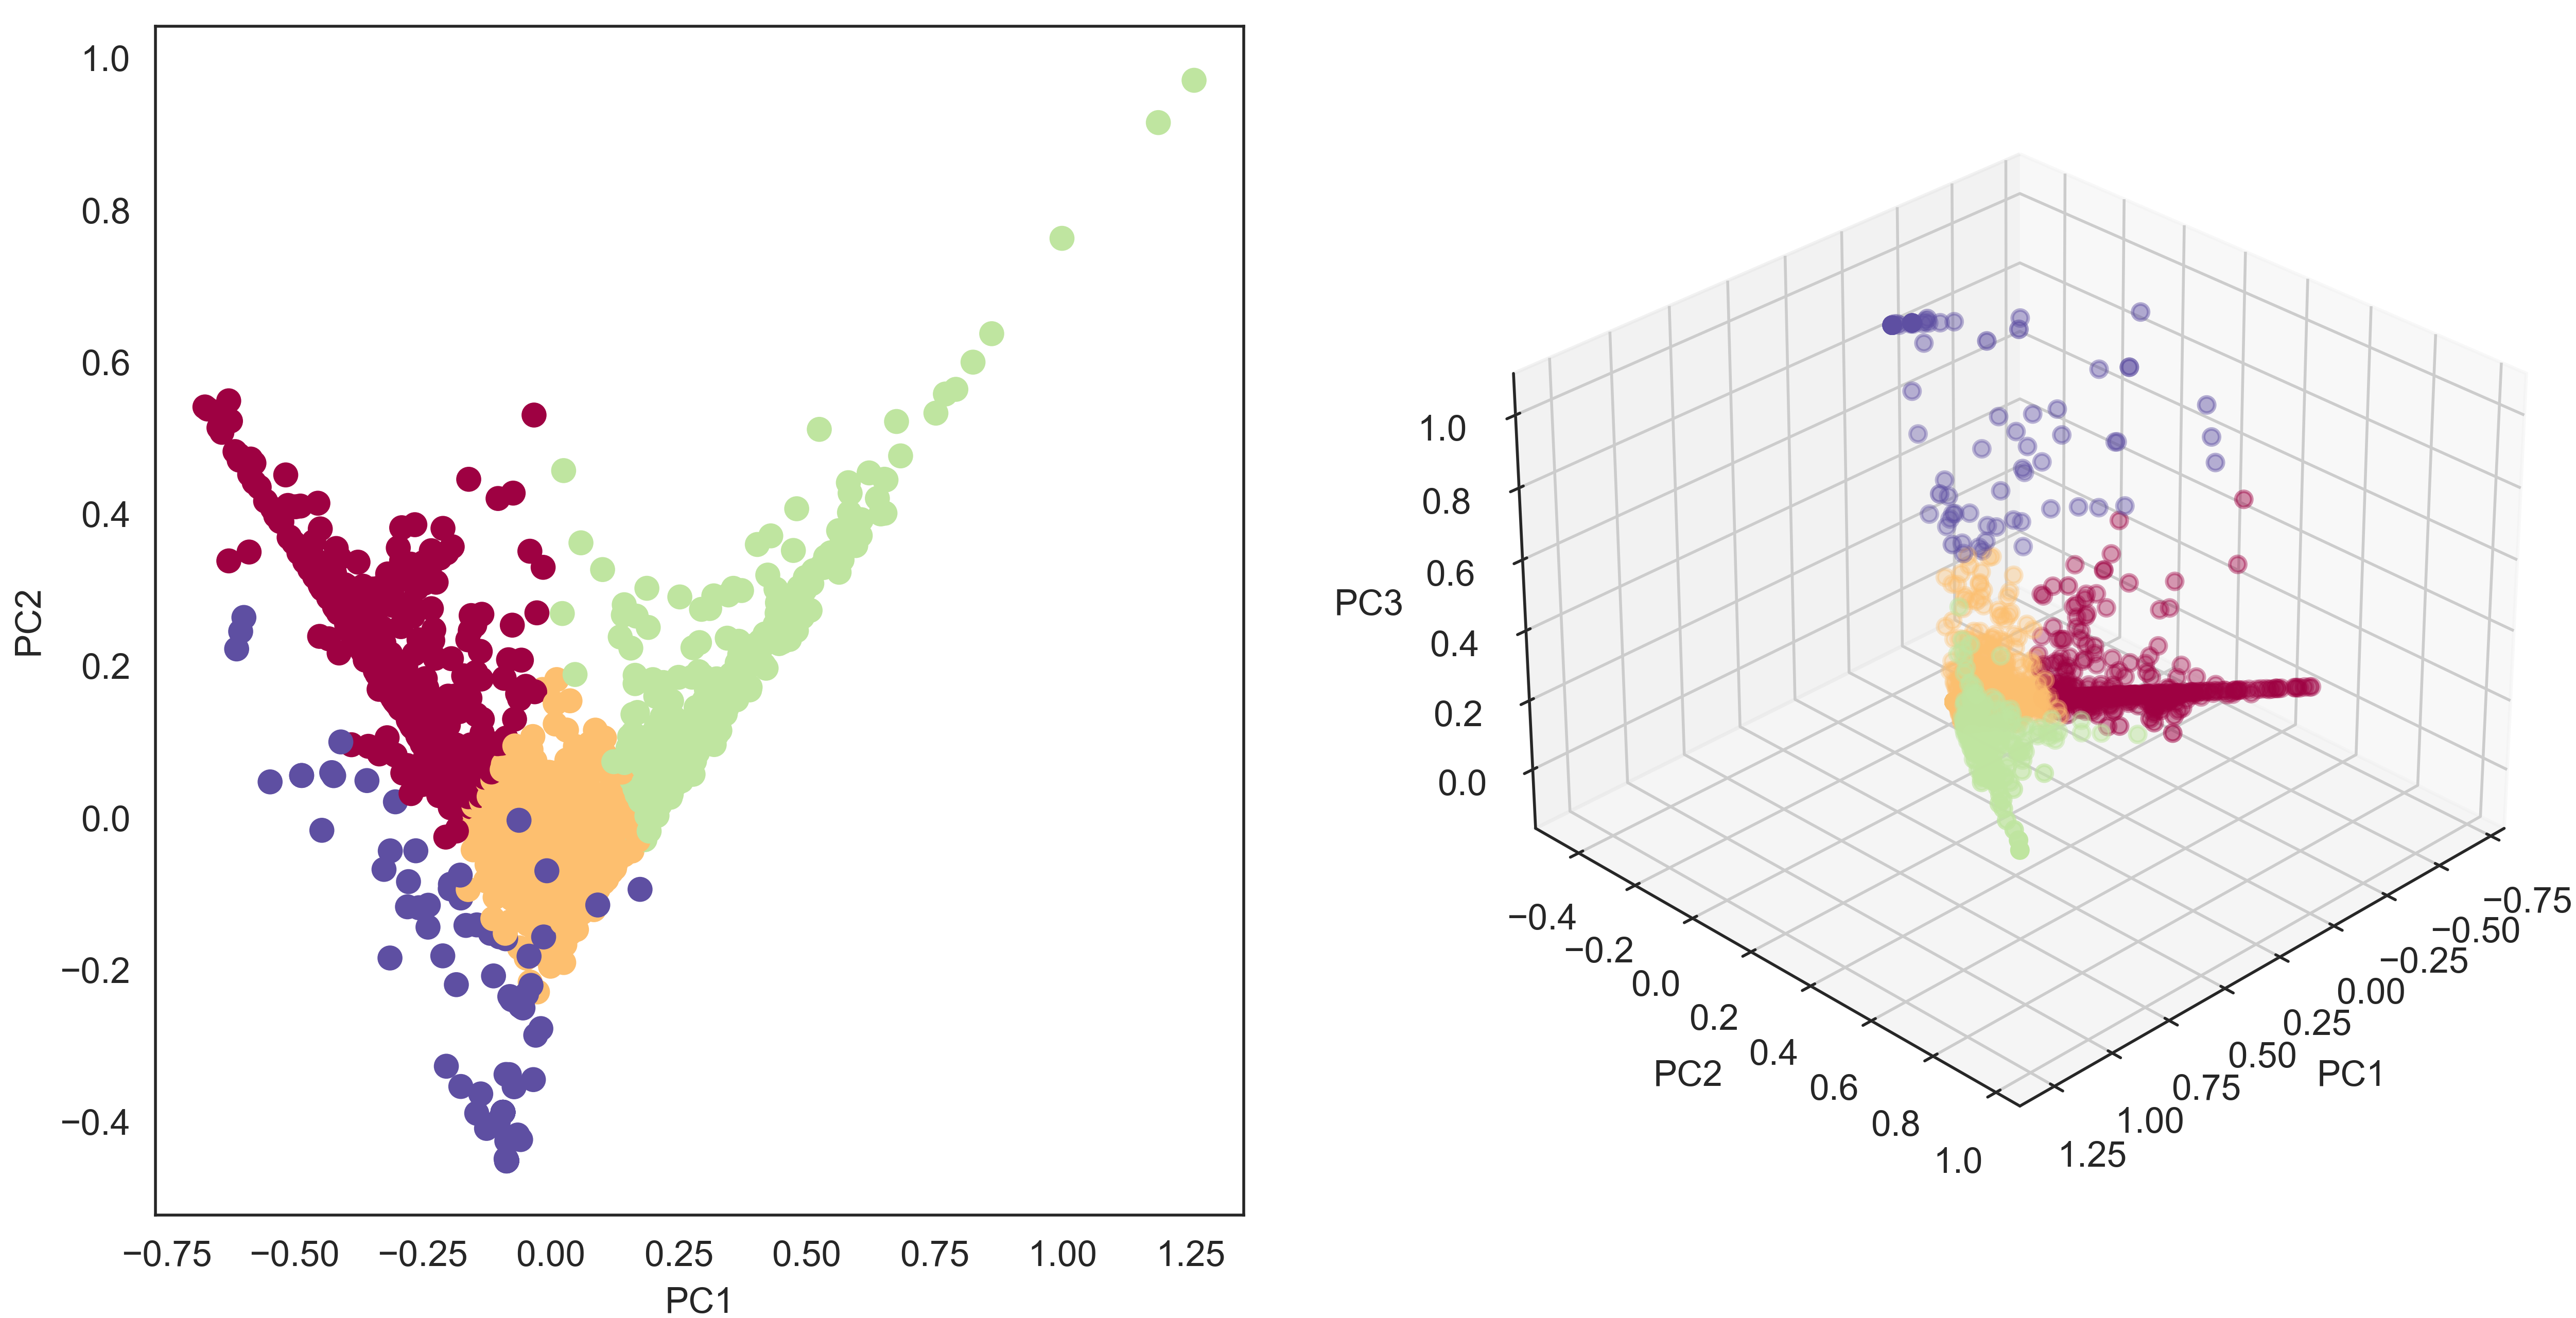
\includegraphics[width=\textwidth]{kmeans-4.png}
  \caption{$k=4$时样本点于主成分空间内投影图}
  \label{4聚类二维三维图}
\end{figure}

通过\figref{4聚类二维三维图}能够看到三千余件商品在此算法下被分为了边界轮廓清晰的4簇,分得的4簇中商品数量分别为2472,605,505,86。为更好的解释每簇代表的商品特性,\tabref{基于4分类的商品特征表}给出了每簇样本特征均值,平均单价和实际成交单价。
\begin{center}
\begin{longtable}{ccccc}
  \caption{基于4分类的商品特征表}
  \label{基于4分类的商品特征表}\\
    \hline
    \textbf{特征名称} & \textbf{分类0} & \textbf{分类1} & \textbf{分类2} & \textbf{分类3}\\
    \hline
    总订单量 & 65.405 & 27.709 & 410.250 & 19.767\\
    总商品购买量 & 713.772 & 329.623 & 5400.194 & 91.453\\
    每单最大购买量 & 108.169 & 51.127 & 352.818 & 934.779\\
    每单最大退货量 & -8.298 & -2.450 & -63.760 & -1052.453\\
    每单平均购买量 & 10.648 & 10.376 & 13.045 & 1.602\\
    每单中位购买量 & 6.822  & 8.314 & 7.650 & 0.372\\
    总销售额 & 1048.650 & 411.496 & 10040.729 & 415.791\\
    每单最大销售额 & 150.436 & 70.703 & 745.860 & 1037.868\\
    每单最大退款额 & -14.374 & -1.463 & -132.547 & -1070.587\\
    每单平均销售额 & 16.223 & 17.971 & 22.872 & 3.023\\
    每单中位销售额 & 11.098 & 14.718 & 13.672 & 2.316\\
    消费者购买人数 & 49.227 & 22.524 & 241.479 & 13.279\\
    最大复购次数 & 4.251 & 2.664 & 15.267 & 2.651\\
    平均复购次数 & 1.265 & 1.214 & 1.689 & 1.453\\
    退货率 & 1.697\% & 2.265\% & 2.128\% & 78.334\%\\
    最大下单间隔 & 33.078 & 151.762 & 18.115 & 67.093\\
    平均订单金额 & 16.033 & 14.851 & 24.475 & 21.034\\
    平均单价 & 1.469 & 1.248 & 1.859 & 4.546\\
    \hline
\end{longtable}
\end{center}

通过\tabref{基于4分类的商品特征表}能够解读出以下几点:
\begin{itemize}
  \item [(1)] 
  分类2中的505件商品的订单量,销售量,销售额,客户受众和平均单价相对其他3类都更优,故认为此类的商品最畅销,盈利能力最强。  
  \item [(2)]
  分类3中的86件商品订单量,销量不佳,且退货率极高,平均单价较高,故认为此类商品的定价上可能过高,或是其他因素,导致其退货率极高。
  \item [(3)]
  分类1中的605件商品的订单量,销量,销售额不佳,但其退货率较为正常,且平均单价较低,认为此类商品属于不畅销商品。
  \item[(4)]
  分类0中商品数量是所有4个分类中最多的,退货率最低,且从各项指标而言都处于平均水品,认为此类商品属于一般畅销,一般盈利水平的商品。 
\end{itemize}

考虑到最畅销的商品订单量有505件,数量相较于总量三千余件仍然比较多,本文想从其中进一步提取畅销、高盈利水平商品。对然$k=5$时平均轮廓系数不是最优,但本文考虑到对商品的针对性分析,故构建了$k=5$的K-Means++分类模型,\figref{5聚类二维三维图}为样本点此时在二维和三维空间内的分布情况。
\begin{figure}[H]
  \centering
  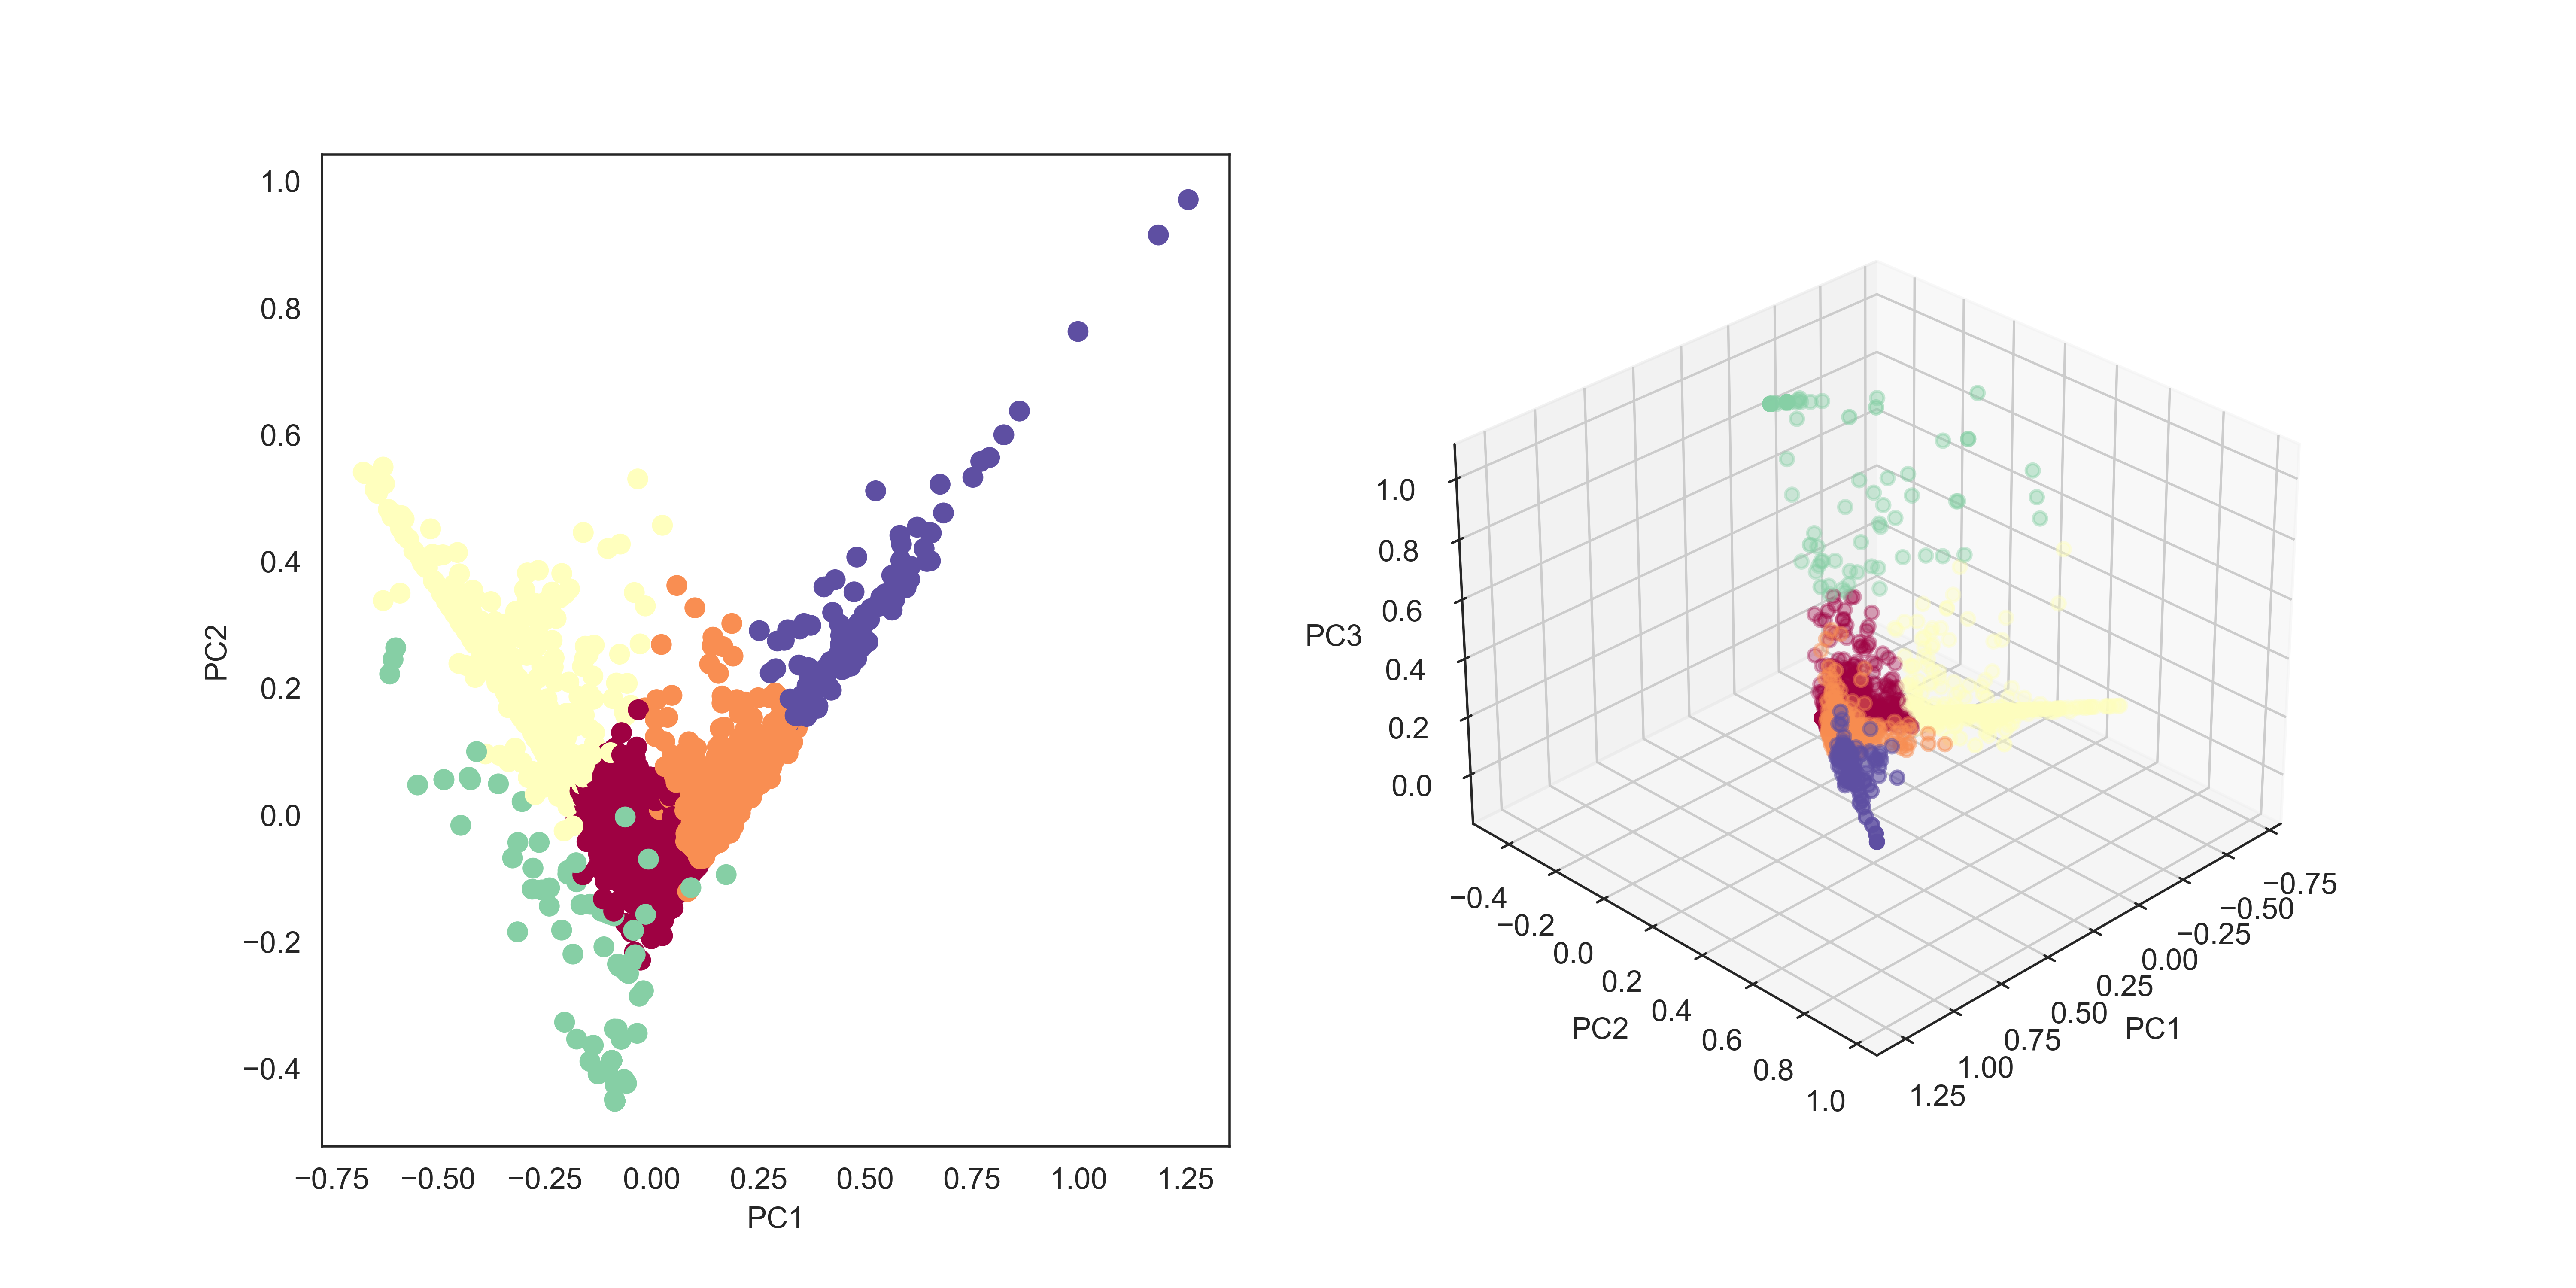
\includegraphics[width=\textwidth]{kmeans-5.png}
  \caption{$k=5$时样本点于主成分空间内投影图}
  \label{5聚类二维三维图}
\end{figure}

根据对比\figref{4聚类二维三维图}和\figref{5聚类二维三维图},$k=5$时分类的改变主要体现在原先最畅销的和一般水平的大部分商品之间又被细分。\tabref{基于5分类的商品特征表}给出了$k=5$时每簇样本的特征均值,平均单价和实际成交单价等特征的平均值。
\begin{center}
\begin{longtable}{c|c|c|c|c|c}
  \caption{基于5分类的商品特征表}
  \label{基于5分类的商品特征表}\\
    \hline
    \textbf{特征名称} & \textbf{分类0} & \textbf{分类1} & \textbf{分类2} & \textbf{分类3} & \textbf{分类4} \\
    \hline
    总订单量 & 229.459 & 29.925 & 699.963 & 42.703 & 20.414\\
    总商品购买量 & 2682.162 & 351.483 & 9990.036 & 468.962 & 95.195\\
    每单最大购买量 & 234.788 & 49.350 & 562.438 & 87.304 & 926.839\\
    每单最大退货量 & -36.327 & -5.455 & -107.204 & -3.512 & -1043.161\\
    每单平均购买量 & 11.743 & 8.290 & 14.405 & 11.047 & 1.647\\
    每单中位购买量 & 7.114  & 6.253 & 8.777 & 7.342 & 0.391\\
    总销售额 & 4590.536 & 443.695 & 19060.822 & 659.529 & 423.521\\
    每单最大销售额 & 458.017 & 66.520 & 1006.544 & 118.731 & 1027.341\\
    每单最大退款额 & -74.622 & -7.166 & -210.038 & -5.273 & -1059.683\\
    每单平均销售额 & 19.190 & 12.981 & 25.799 & 17.333 & 3.153\\
    每单中位销售额 & 11.944 & 9.964 & 15.668 & 12.446 & 2.376\\
    消费者购买人数 & 153.272 & 24.073 & 366.854 & 33.851 & 13.826\\
    最大复购次数 & 10.499 & 2.723 & 21.124 & 3.353 & 2.678\\
    平均复购次数 & 1.520 & 1.214 & 1.623 & 1.226 & 1.451\\
    退货率 & 2.059\% & 2.253\% & 2.067\% & 1.587\% & 77.901\%\\
    最大下单间隔 & 18.781 & 162.960 & 17.088 & 38.801 & 66.736\\
    平均订单金额 & 20.006 & 14.827 & 27.231 & 15.444 & 20.747\\
    平均单价 & 1.712 & 1.262 & 1.908 & 1.406 & 4.449\\
    \hline
\end{longtable}
\end{center}

通过\tabref{基于5分类的商品特征表}能够解读出几点:
\begin{itemize}
  \item [(1)] 
  分类2中的137件商品相较于$k=4$时分类2中的商品数量有所下降,订单量,销售量,销售额,客户受众和平均单价不仅优于其他4类,且也优于k=4时分类2的相关指标,故认为此类的商品是对之前分类的畅销,高盈利商品的进一步提炼,属于销量,盈利能力都极好的产品。  
  \item [(2)]
  分类4中的87件商品订单量,特点与$k=4$时的分类3中商品特征一致,属于单价超高,退货率极高的商品。
  \item [(3)]
  分类1中的505件商品的订单量,销量,销售额不佳,但其退货率较为正常,且平均单价较低,认为此类商品属于不畅销商品。
  \item[(4)]
  分类3中商品数量是所有5个分类中最多的,退货率最低,且从各项指标而言都处于平均水品,认为此类商品属于一般畅销,一般盈利水平的商品。 
  \item[(5)]
  分类0中的798件商品主要来自$k=4$时的畅销和普通商品,此类商品各项水平较为均衡,销量,但销量和销售额也超普通商品一个数量级,认为此类商品为略逊于分类2中的商品但销量,盈利水平都相当不错的产品。 
\end{itemize}

此外,本文还尝试了采用DBSCAN的方法尝试分类上述模型。经过对$eps$和$MinPts$的多轮实验,得到最优结果为$eps=0.1$,$MinPts=10$。此时模型分类结果如\figref{DBSCAN聚类二维三维图}所示:
\begin{figure}[H]
  \centering
  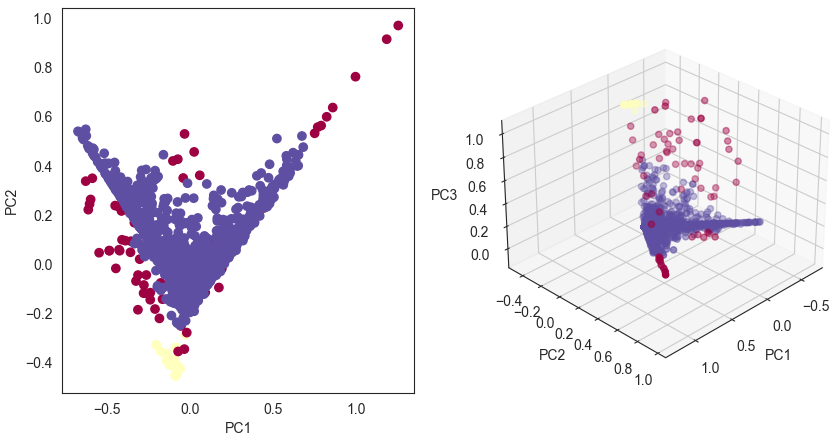
\includegraphics[width=\textwidth]{dbscan.png}
  \caption{DBSCAN聚类样本点于主成分空间内投影图}
  \label{DBSCAN聚类二维三维图}
\end{figure}

通过DBSCAN的方法很难像K-Means++一样对商品在主成分构成的三维空间内实施有效划分,故本人认为$k$取值为5的K-Means++算法能够在保证算法的有效性前提下提供最好的可解释性。

根据上述分析,\tabref{商品聚类信息表}为本文根据聚类给出的部分商品ID信息(以StockCode排序)
\begin{center}
\begin{longtable}{c|c|c|l}
  \caption{商品聚类信息表}
  \label{商品聚类信息表}\\
    \hline
    \textbf{分类名} & \textbf{分类数量} & \textbf{商品特征}& \textbf{StockCode(从小到大排序,取前10个)}\\
    \hline
    0 & 798 & 较畅销,盈利水平中上 & \begin{tabular}[c]{@{}l@{}}
      10135, 15036, 16237, 17003, 20668, \\20674, 20675, 20676, 20677, 20679
    \end{tabular} \\
    1 & 505 & 不畅销,低盈利水平 & \begin{tabular}[c]{@{}l@{}}
      10080, 16048,	16052, 16054,	17174, \\20653,	20661, 20662, 20663, 20670
    \end{tabular}\\
    2 & 137 & 最畅销,高盈利水平 & \begin{tabular}[c]{@{}l@{}}
      20685, 20712, 20719, 20723, 20724, \\20725, 20726, 20727, 20728, 20914
    \end{tabular}\\
    3 & 2141 & 普通商品 & \begin{tabular}[c]{@{}l@{}}
      10002, 10120, 10125, 10133, 11001, \\15030, 15034, 15039, 16008, 16010
    \end{tabular} \\
    4 & 87 & 退货率极高,单价超高 & \begin{tabular}[c]{@{}l@{}}
      20703, 20793, 20821, 20857, 20901, \\20957, 21144, 21275, 21412, 21645
    \end{tabular}\\
    \hline
\end{longtable}  
\end{center}

\section{平台用户价值分析}

\subsection{RFM模型介绍及改进}

RFM模型是用来描述客户价值的客户群体的分类模型。R,F,M分别为3个英文单词的缩写。R(Rencency)指的是客户最近一次消费距离现在的时间,F(Frequency)指的是某一段时间内客户消费的频率,M(Monetary)指的是某一段时间内客户消费的金额。其中,客户最近一次消费的时间离现在越短,则R越小,客户的价值就越高;客户购买的频率越高,则F越大,客户的价值就越高;客户消费的金额越大,则M越大,客户的价值也会越高。通过这3个不同的维度来综合评价一个客户的价值状况,根据实际不同的业务背景下,可稍加修改。由于对每个维度都设定一个阈值,可以是中位数,平均数,又或者是根据具体的业务场景来设定符合各自本身的阈值。大于该阈值的用户则将其对应维度的值记为1,否则记为0。每个阈值可把客户这个样本分为两类,那么在3个维度下,客户就可以分为8个分类,即2的3次方幂。如\tabref{用户类别划分表}所示:
\begin{center}
  \begin{longtable}{c|c|c|c}
    \caption{用户类别划分表}
    \label{用户类别划分表}\\
      \hline
      \textbf{用户价值分类} & \textbf{R值} & \textbf{F值} & \textbf{M值} \\
      \hline
      高价值客户 & 1 & 1 & 1 \\
      重要保持客户 & 0 & 1 & 1 \\
      重要发展客户 & 1 & 0 & 1 \\
      重要挽留客户 & 0 & 0 & 1 \\
      一般价值客户 & 1 & 1 & 0 \\
      一般保持客户 & 0 & 1 & 0 \\
      一般发展客户 & 1 & 0 & 0 \\
      潜在客户 & 0 & 0 & 0 \\
      \hline
  \end{longtable}
  \end{center}

由于本文提取的有关用户的特征较多,不便于直接构建解释性较强的R值,F值和M值。故本文将根据已提取的基于用户的特征,综合从用户的消费量,退单率和消费间隔等角度出发,针对RFM模型中三个指标的含义,重新构建新的指标。本文首先将针对即将用到的指标进行标准化以避免不同量纲对指标构建的影响。具体指标如\tabref{改进指标}所示:
\begin{center}
  \begin{longtable}{c|l}
    \caption{改进RFM指标}
    \label{改进指标}\\
    \hline
    \textbf{改进指标} & \textbf{计算方式} \\
    \hline
    R & 最近消费间隔-最初最终消费间隔 \\
    F & 下单率-退货率\\
    M & 消费总金额+有效消费金额 \\
    \hline
  \end{longtable}
\end{center}

\subsection{基于RFM的用户价值分类模型构建}
本文在经过上述标准化和改进R,F,M值的构建后,本文依据样本中位数对每个样本的所属分类进行划分。为检验本文划分的指标的效果,本文对获得的8个分类中的客户的特征进行求均值的处理。求得的均值能够很好反应当前分类内的样本的R,F,M值特征。本文做出了基于分类的用户特征雷达图如\figref{用户特征图}:
\begin{figure}[H]
  \centering
  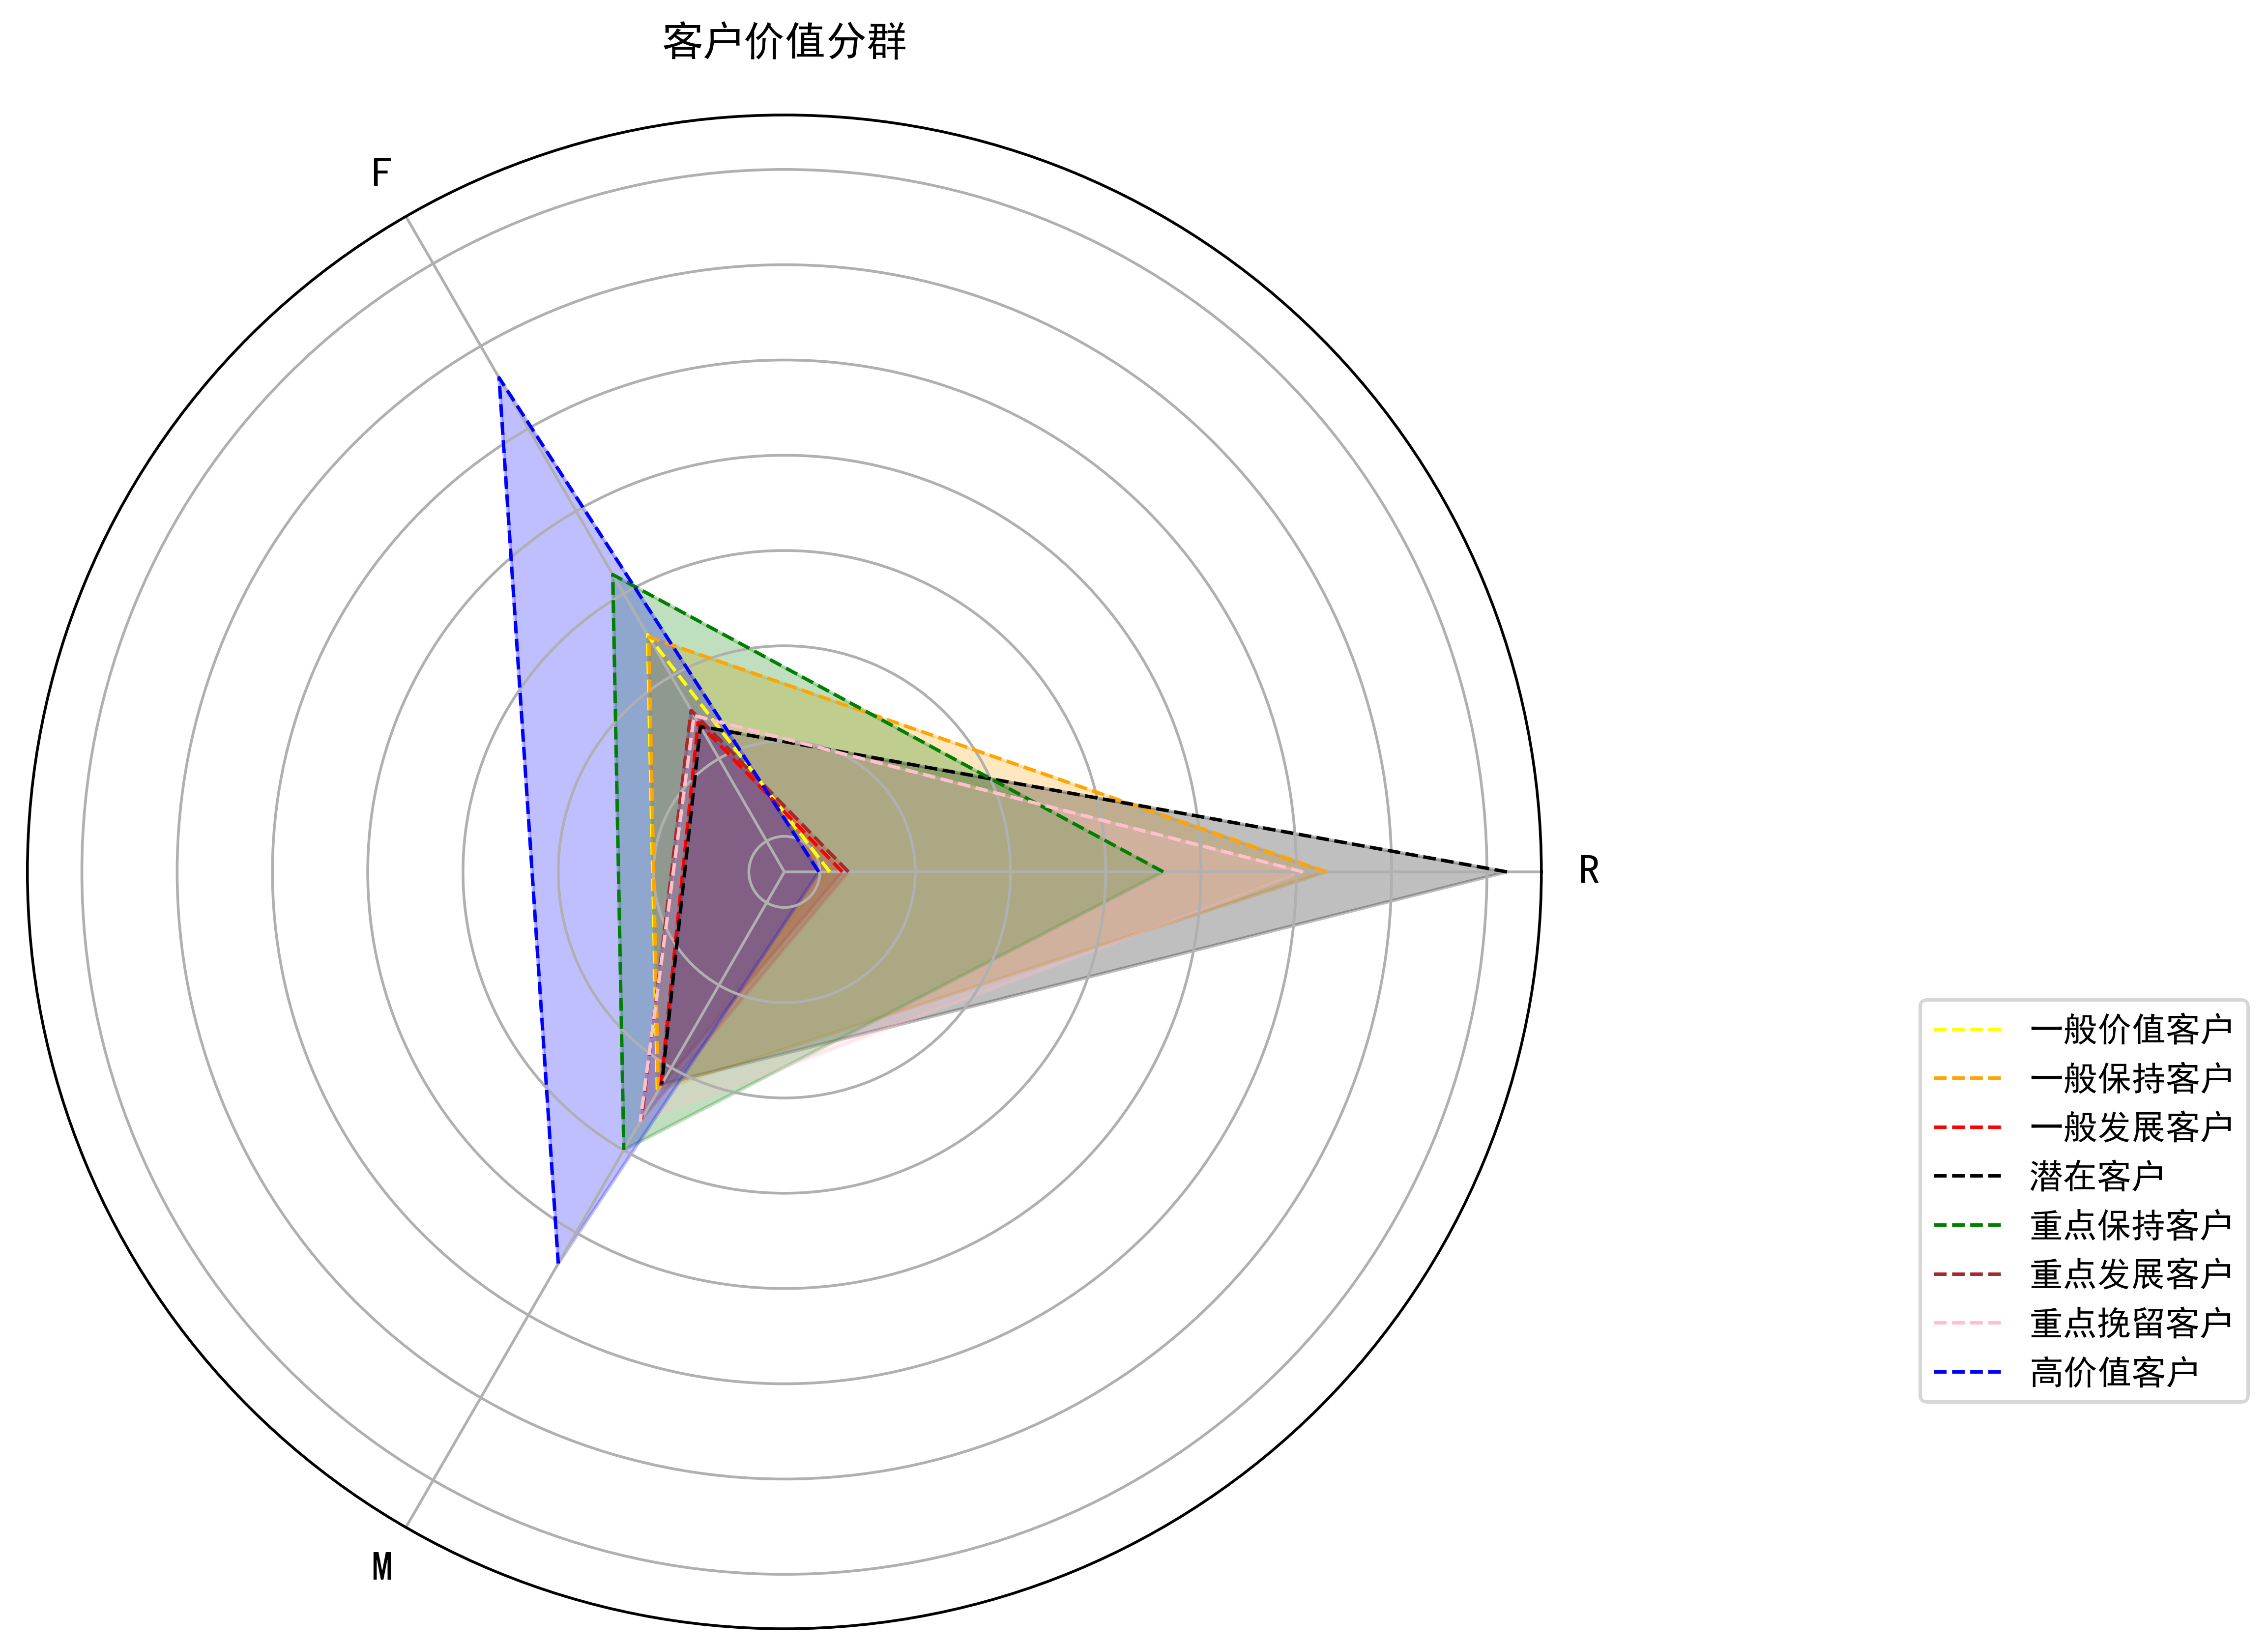
\includegraphics[width=\textwidth]{rfm.png}
  \caption{基于分类的用户RFM特征图}
  \label{用户特征图}
\end{figure}

可以看到高价值用户在反应消费频率和金额的F和M指标上都显著高于其他分类客户的均值。而潜在用户在反应消费间隔的R值上显著高于其余分类的用户,在其余两个维度上得分较低,代表其在该平台消费时间间隔较长,而消费频率和金额较低,符合其潜在用户的定义。划分出的用户CustomerID在\tabref{用户分类信息表}中给出:
\begin{center}
  \begin{longtable}{c|c|l}
    \caption{用户分类信息表}
    \label{用户分类信息表}\\
      \hline
      \textbf{分类名} & \textbf{分类数量} & \textbf{CustomerID(从小到大排序,取前20个)}\\
      \hline
      高价值用户 & 1324 & \begin{tabular}[c]{@{}l@{}}
        12347	12352	12356	12359	12360	12362	12364	12370	12380	12381\\
        12388	12395	12406	12407	12408	12415	12417	12421	12427	12428
      \end{tabular} \\
      重要保持用户 & 478 & \begin{tabular}[c]{@{}l@{}}
        12348	12372	12379	12383	12393	12399	12409	12410	12412	12413 \\
        12422	12423	12434	12455	12457	12468	12502	12507	12520	12530
      \end{tabular} \\
      重要发展用户 & 147 & \begin{tabular}[c]{@{}l@{}}
        12349	12357	12371	12374	12397	12398	12438	12446	12465	12475	\\
        12526	12589	12603	12611	12612	12630	12631	12638	12646	12658
      \end{tabular} \\
      重要挽留用户 & 217 & \begin{tabular}[c]{@{}l@{}}
        12354	12377	12378	12394	12405	12418	12424	12425	12435	12453	\\
        12458	12461	12497	12501	12510	12514	12516	12534	12535	12545
      \end{tabular} \\
      一般价值用户 & 166 & \begin{tabular}[c]{@{}l@{}}
        12384	12452	12498	12504	12577	12628	12654	12787	12808	12879	\\
        12895	12933	12990	12993	13058	13066	13079	13145	13171	13247
      \end{tabular} \\
      一般保持用户 & 209 & \begin{tabular}[c]{@{}l@{}}
        12365	12414	12493	12527	12559	12579	12593	12601	12649	12680	\\
        12695	12797	12811	12829	12845	12888	12891	12908	12930	12987
      \end{tabular} \\
      一般发展用户 & 558 & \begin{tabular}[c]{@{}l@{}}
        12375	12391	12403	12430	12445	12448	12454	12479	12491	12508	\\
        12522	12531	12532	12538	12544	12552	12556	12571	12572	12581
      \end{tabular} \\
      潜在用户 & 1232 & \begin{tabular}[c]{@{}l@{}}
        12346	12350	12353	12355	12358	12361	12363	12373	12386	12390	\\
        12401	12402	12420	12426	12436	12441	12447	12450	12489	12492
      \end{tabular} \\
      \hline
  \end{longtable}  
  \end{center}

\section{基于图神经网络的推荐系统}

\subsection{推荐系统简介}

推荐系统如今对业界时一个十分重要的研究领域,包括电商销售,文娱网站等都十分依赖推荐系统以提升其营业水平。早在21世纪初,雅虎,谷歌,脸书等国外互联网企业就开始通过推荐系统为用户精准推送内容或商品,近年来,阿里巴巴,字节跳动等互联网公司也通过为用户提供个性化的推荐而在商业上获得了较大成功。

推荐系统的一个重要研究方向即是本文所关注的基于历史信息的商品个性化排序推荐。其任务就是要根据用户历史数据等信息,为平台每个用户生成一列物品排序。在前深度学习时代,传统推荐模型主要由协同过滤(CF)模型族,Logistic回归模型族,因子分解机(FM)模型族和各类组合模型构成。其中的不少模型尤其是协同过滤(CF)至今仍是研究推荐系统的重要基础。随着近年来深度学习的出现,其在推荐系统中也扮演了十分重要的作用。从简单的单层神经网络AutoRec的运用到深度神经网络Deep Crossing,再到各类特征向量交叉,各种模型组合等,以及近来图神经网络(GNN)的应用,为推荐系统的发展提供了诸多可行方向。

最早的推荐系统算法一般只考虑用户和物品的交互信息,随着该领域研究的推进,越来越多的用户历史数据,标签数据等得以得到运用,这也帮助提升了推荐系统算法的推荐效果。本文将充分运用已有的交互信息和用户,商品特征以获得更好的推荐结果。

\subsection{BPR个性化排序推荐模型}
在早年间,由于推荐系统往往被用于预测用户是否会浏览某个内容或是购买某种物品,算法并没有针对排序问题单独优化。由于推荐系统中用户、物品交互数据往往十分稀疏,导致原有的算法在排序问题中,无法有效的区分处理负反馈样本和缺失值,导致排序效果不佳。Rendle等的\cite{rendle_bpr_2009}和Li等的\cite{li_tag-aware_2019}提出的贝叶斯个性化推荐排序标准和优化方法的构建就是针对排序这一问题的。

令$U$为全体用户的集合,$I$为全体物品的集合,所有的隐式反馈记为$S \subseteq U \times I$,记为正反馈$x_{uij}$,即用户与该产品产生了交互。所有的$(U \times I) \backslash S$统一视为负反馈。记$\succ_u \subset I^2$为用户$u$所有物品的排序,则$i \succ_u j$代表用户$u$相较于物品$j$更倾向于物品$i$。在贝叶斯个性化排序模型中,训练集记为$D_S : U \times I \times I$:
\begin{equation}
  D_S = \{ (u, i, j) | i \in I_u^+ \wedge j \in I \backslash I_u^+\}
\end{equation}

其中$I_u^+ = \{i \in I: (u, i) \in S\}$,$D_S$中的样本表示用户相较于物品$j$更倾向于物品$i$。基于上述的训练集,构建的BPR优化标准是要根据上述的训练集优化模型参数$\Theta$,根据贝叶斯思想,有参数条件概率$p(\Theta|\succ_u) \varpropto p(\succ_u|\Theta)p(\Theta)$。要求上述条件概率分布,首先要对所有用户求$p(\succ_u|\Theta)$。
\begin{equation}
  \prod_{u \in U}p(\succ_u|\Theta)=\prod_{(u, i, j) \in U \times I \times I}p(i \succ_u j|\Theta)^{\delta((u, i, j)\in D_S)} \cdot (1- p(i \succ_u j|\Theta))^{\delta((u, i, j) \notin D_S)}
\end{equation}

其中$\delta$为示性函数。由于观测中,用户的偏好概率函数难以观测,故使用激活函数激活观测的正反馈观测值近似:
\begin{equation}
  p(i \succ_u j|\Theta) \approx \sigma(\hat{x_{uij}}(\Theta))
\end{equation}

上式中的$\sigma$为$sigmoid$激活函数。由于$\Theta$的先验概率为$N(0, \Sigma_{\Theta})$,则可以得到贝叶斯优化标准$BPR-OPT$:
\begin{equation}
  \begin{split}
    max \ BPR-OPT &= ln p(\Theta|\succ_u) = ln p(\succ_u|\Theta)p(\Theta) \\
  &= \sum_{(u, i, j)\in D_S}ln\sigma(\hat{x_{uij}}) - \lambda_{\Theta}\parallel \Theta \parallel^2
  \end{split}
\end{equation}

上述贝叶斯优化标准就是最大化模型参数的似然函数。由于在深度学习中最小化模型损失函数采用的是梯度下降法,故为了方便,上述优化标准也等价于:
\begin{equation}
  min \ L = -\sum_{(u, i, j)\in D_S}ln\sigma(\hat{x_{uij}}) + \frac{\lambda}{2}(\sum_{u \in U}\parallel U_u \parallel_2^2+\sum_{i \in I}\parallel I_i \parallel_2^2)
\end{equation}

其中$\lambda$为参数的正则化参数。另外在实际运算中,$\hat{x_{uij}}$很多时候无法之间观测,考虑到其表示用户选择偏好的内在含义,故其可以通过$\hat{x_{uij}} = \hat{x_{ui}}-\hat{x_{uj}}$计算得到,其中$\hat{x_{ui}}$在传统协同过滤模型中是通过矩阵分解得到的,即$\hat{x_{uij}} = U_uV_i^T$。
% 为了进一步缓解过拟合问题,提升推荐销量,本文采取基于用户图的正则化项:
% \begin{equation}
%   \begin{split}
%     min \ L &= -\sum_{(u, i, j)\in D_S}ln\sigma(U_uV_i^T-U_uV_j^T) + \frac{\lambda}{2}(\sum_{u \in U}\parallel U_u \parallel_2^2+\sum_{i \in I}\parallel I_i \parallel_2^2) \\
%     &+\frac{\gamma}{2}(\sum_{u\in U}\parallel U_u-\sum_{v\in N(u)}sim(u,v)U_v / \sum_{v\in N(u)}sim(u,v) \parallel)
%   \end{split}
% \end{equation}

根据上述获得的目标损失函数,模型的优化就是对其采用随机梯度下降法。
\begin{gather}
  \delta = -\frac{\partial ln\sigma(\hat{x_{uij}})}{\partial(\hat{x_{uij}})} = -(1-\sigma (\hat{x_{uij}})) \\
  \frac{\partial L}{\partial U_u} = \delta(V_i-V_j)+\lambda U_u , \quad U_u \leftarrow U_u - \eta \frac{\partial L}{\partial U_u} \\
  \frac{\partial L}{\partial V_i} = \delta U_u+\lambda V_i , \quad V_i \leftarrow V_i - \eta \frac{\partial L}{\partial V_i} \\
  \frac{\partial L}{\partial V_j} = \delta (-U_u)+\lambda V_j , \quad V_j \leftarrow V_j - \eta \frac{\partial L}{\partial V_j} 
\end{gather}

通过随机梯度下降法,即可得到参数$\Theta$的估计。通过此估计即可分别计算用户$u$对商品$i$的偏好程度并最终生成用户个性排序推荐。

\subsection{NGCF及LGCN推荐系统算法}
随着GNN在节点分类,连接预测等领域应用的展开,基于图神经网络的推荐系统算法也随之产生。在基于图的推荐系统中,以电商平台为例,所有的用户和商品都被视作图神经网络中的节点,节点的分类可以是多种多样的。用户对商品的查看,收藏和购买的行为都可被视作连接节点的边,具体根据任务目标决定。图神经网络能够高效的将相似节点进行分类,从而实现对未知节点,或者边的预测,而这就与推荐系统中相似用户选择相似商品的假设不谋而合。

图卷积神经网络(GCN)的得名来源于卷积神经网络(CNN)的思想。卷积神经网络是在二维平面对节点做卷积运算,而图神经网络将这一运算拓展至三维空间。Wang等提出的\cite{wang_neural_2019}NGCF(Neural Graph Collaborative Filtering)是一个将GCN与CF结合的模型。GNN中计算最终输出过程中起主要作用的是特征信息聚合与传递。NGCF模型中,商品$i$向用户$u$传递的信息为:
\begin{equation}
  m_{u \leftarrow i} = \frac{1}{\sqrt{|N_u||N_i|}}(W_1e_i+W_2(e_i \odot e_u))
\end{equation}

其中$W_1$和$W_2$为可训练权重参数,$\odot$表示元素积,$N_u$和$N_i$表示用户$u$和商品$i$邻域的节点个数。即在消息传递的过程中用户接受来自于近邻商品的信息。用户$u$在下一层的特征向量可以通过带激活函数的特征传递函数计算得到:
\begin{gather}
  e_u^{(k+1)} = \sigma(W_1e_u^{(k)}+\sum_{i\in N_u}\frac{1}{\sqrt{|N_u||N_i|}}(W_1e_i^{(k)}+W_2(e_i^{(k)}\odot e_u^{(k)}))) \\
  e_i^{(k+1)} = \sigma(W_1e_i^{(k)}+\sum_{u\in N_i}\frac{1}{\sqrt{|N_u||N_i|}}(W_1e_u^{(k)}+W_2(e_u^{(k)}\odot e_i^{(k)})))
\end{gather}

式中$e_u^{(k)}$的上标代表神经网络的层数,在经过所有的$L$层的信息传递与表征聚合后,模型通过连接函数将前面的所有层表征结合即可得到最终的用户或商品表征输出。目标用户与商品的输出表征内积即可得到该用户对特定商品的偏好得分。此种方法的使用有效提升了协同过滤系列算法的表现能力。但GCN其最初的应用领域为基于图的节点分类任务,节点通常拥有充分的输入特征信息,但在一般推荐系统算法的数据集中,用户商品的交互常采用独热编码,数据稀疏性大,故复杂的信息传递和特征聚合函数在NGCF的实际应用中反而为训练速度和精度带来的负面影响。故在此基础上,He等人提出的\cite{he_lightgcn_2020}LGCN简化了相关函数的形式。其中信息聚合和特征传递过程中的可训练参数$W$和内积操作被舍弃,变为直接相加:
\begin{gather}
  e_u^{(k+1)} = \sum_{i\in N_u}\frac{1}{\sqrt{|N_u||N_i|}}e_i^{(k)} \\
  e_i^{(k+1)} = \sum_{u\in N_i}\frac{1}{\sqrt{|N_u||N_i|}}e_u^{(k)}
\end{gather}

为了避免表征在卷积计算的过程中发生量纲上的变化,式中$\frac{1}{\sqrt{|N_u||N_i|}}$的部分沿用了NGCF的形式。由此LGCN模型中仅剩的可训练参数则是用户和商品节点的初始表征。在经过$k$层神经网络后,用户和商品表征最终的输出为:
\begin{equation}
  e_u = \sum_{k=0}^K\alpha_ke_u^{(k)} \ ; \ e_i = \sum_{k=0}^K\alpha_ke_i^{(k)}
\end{equation}

式中$\alpha_k$代表每层表征在最终输出中的权重系数,其可以是一个可训练的参数,但在推荐系统中,其统一被设定为$\frac{1}{K+1}$。最终目标用户对特定商品的偏好为:
\begin{equation}
  \hat{x_{ui}} = e_u^Te_i
\end{equation}

根据用户对商品偏好的评分和BPR个性化排序推荐算法的思想,即可得到用户的排序推荐列表。

\subsection{WideGCN个性化排序推荐}
本文已经介绍了图卷积网络在推荐系统中应用的最主要的两个算法:NGCF和LGCN。这两个基于协同过滤类型的算法难以引入用户和商品的旁信息(side information),而这些旁信息对提升推荐效果有着非常重要的作用。上述算法都只采用用户与商品的历史交互信息,而在前文中已经完成了的基于商品和用户的特征工程里,本文已经对每个商品和用户提取了16条特征信息。本文考虑有效引入上述特征,用以帮助用户和商品表征的学习。在训练LGCN模型的同时,本文分别为用户特征和商品特征构建两个全连接神经网络,用作学习用户与商品特征。本文基于使用深度神经网络构建用户-商品对旁信息特征提取,并与LightGCN信息聚合。从而扩展原本对于用户和商品信息的表征。

在WideGCN中的轻量化图卷积部分,输入的数据为用户消费记录,每个用户和商品都会有一个随机生成的初始表征。每个节点在每层神经网络中接收与其连结的节点向其传递的表征,并通过聚合函数将信息进行聚合并传递至下一层。这样的信息传递机制赋予了用户和商品学习与其关联节点信息的能力。

与轻型卷积并列的,本文构建两个全连接神经网络分别用于学习用户和商品的表征。该神经网络将前文提取到16维基于用户和商品的特征作为输入,输出一个与LGCN的表征大小一致的用户、商品表征,分别与图神经网络的输出表征结合后,即可得最终的表征信息。

\section{基于图神经网络的推荐系统模型构建及结果分析}
\subsection{实验设置}
本文的实验数据来自于某礼品批发平台一年内的订单信息,本文将其中非商品交易信息(例如邮费,银行收费)剔除后,实际的用户交易信息共379128条,商品个数3668条,顾客人数4331人,数据稀疏度为97.61\%。

至于模型选择,本文将以选取Popularity推荐算法作为基线(Baseline)模型,同时构建BPR,NGCF,LGCN和WideGCN模型,通过召回率(Recall),准确率(Precision),命中率(Hit),归一化折损累计增益(NDCG)和平均倒序排名(MRR)对模型的表现进行评估。

在模型训练集,验证集和测试集的划分上,本文将根据时间排序前60\%的数据列为训练集,后20\%的数据作为测试集,其余的20\%数据作为验证集。按照时间顺序划分数据集的好处在于避免神经网络在训练过程中具备超越时空的学习的能力。随机划分数据集虽然可能带来评价指标上的提升,但在未知数据上可能表现糟糕。

除了Pop模型,本文对其余所有的模型在多个随机种子下进行了超参数实验,用以确定使各自模型表现最好的参数,学得最优参数如\tabref{超参数表}所示:
\begin{center}
  \begin{longtable}{c|l}
    \caption{模型超参数表}
    \label{超参数表}\\
      \hline
      \textbf{模型} & \textbf{超参数取值} \\
      \hline
      BPR & Learning Rate: 0.001, Regression Weight: 0.0001 \\
      NGCF & \begin{tabular}[c]{@{}l@{}}
        Learning Rate: 0.001, Regression Weight: 0.1, Node Dropout: 0,\\
        Message Dropout: 0
      \end{tabular}\\
      LGCN & Learning Rate: 0.005, Regression Weight: 0.01, Number of Layers: 3 \\
      WideGCN & \begin{tabular}[c]{@{}l@{}}
        Learning Rate: 0.005, Regression Weight: 0.01, Number of Layers: 3,\\
        Dropout Probability: 0.3
      \end{tabular}\\
      \hline
  \end{longtable}
  \end{center}

为保证训练效率,本文的设定训练Batch size为2048,同时训练轮数设计有早停机制。

\subsection{结果分析}
本文的实验是基于Pytorch和基于其的Recbole\cite{zhao_recbole_2021}框架构建的。根据之前最优超参数的实验结果,选取在多轮随机种子下模型的最优表现。\tabref{模型实验指标结果}为各模型的最优结果的指标表。
  \begin{table}[!htb]
    \centering
    \caption{模型表现对比表}
      \huge
      \begin{tabular}{C{2cm}|C{1.5cm}|C{1.5cm}|C{1.5cm}|C{1.5cm}|C{1.5cm}}
      \hline
      \textbf{指标名称} & \textbf{Baseline} & \textbf{BPR} & \textbf{NGCF} & \textbf{LGCN} & \textbf{WideGCN} \\
      \hline
      Recall@10 & 0.0384 & 0.1025 & 0.0999 & 0.0997 & 0.1044\\
      Recall@20 & 0.0587 & 0.1547 & 0.1525 & 0.1556 & 0.1581\\
      Pricision@10 & 0.0437 & 0.0952 & 0.0927 & 0.0928 & 0.0964\\
      Pricision@20 & 0.0381 & 0.0802 & 0.0790 & 0.0795 & 0.0815\\
      Hit@10 & 0.2875 & 0.4218 & 0.4202 & 0.4185 & 0.4162 \\
      Hit@20 & 0.3671 & 0.5334 & 0.5343 & 0.5322 & 0.5377 \\
      Ndcg@10 & 0.0564 & 0.1297 & 0.1272 & 0.1292 & 0.1328 \\
      Ndcg@20 & 0.0594 & 0.1393 & 0.1369 & 0.1397 & 0.1422 \\
      Mrr@10 & 0.1215 & 0.2083 & 0.2073 & 0.2125 & 0.2141 \\
      Mrr@20 & 0.1273 & 0.2159 & 0.2153 & 0.2204 & 0.2225 \\
      \hline
      \end{tabular}
    \label{模型实验指标结果}
  \end{table}

  从\tabref{模型实验指标结果}可以观测到,所有的BPR,NGCF,LGCN和WideGCN的模型表现较Baseline模型都有较大提升。且WideGCN模型的表现稳定的优于BPR和LGCN,在Recall和Ndcg这两个最重要的指标上,WideGCN较其余模型的提升如\tabref{WGCN提升表}:
  \begin{table}[!htb]
    \centering
    \caption{WideGCN模型表现提升率}
      \huge
      \begin{tabular}{C{2cm}|C{1.5cm}|C{1.5cm}|C{1.5cm}|C{1.5cm}}
      \hline
      \textbf{指标名称} & \textbf{Baseline} & \textbf{BPR} & \textbf{NGCF} & \textbf{LGCN} \\
      \hline
      Recall@10 & 171.88\% & 1.85\% & 4.50\% & 4.71\% \\
      Recall@20 & 169.34\% & 2.20\% & 3.67\% & 1.61\% \\
      Ndcg@10 & 135.46\% & 2.39\% & 4.40\% & 2.79\% \\
      Ndcg@20 & 139.39\% & 2.08\% & 3.87\% & 1.79\% \\
      \hline
      \end{tabular}
    \label{WGCN提升表}
  \end{table}

  根据\tabref{WGCN提升表}的结果显示WideGCN模型引入的商品、用户特征信息对于图神经网络推荐系统的推荐效果提升都是有效的,不论对于Top10还是Top20的排序推荐任务,模型的较其余模型的表现提升的稳定的且显著的。

  随后本文探索运用已训练出的模型对686名顾客的潜在喜好商品进行预测,在预测的过程中,本文发现只有645名用户在过去一年间有过下单记录,其余41名用户是缺少下单记录的。故本文将对645名有过历史下单记录的用户采用基于WideGCN的个性化排序推荐模型预测他们对商品的潜在偏好。对剩余的41名用户,本文运用Popularity及本文的基线模型对他们的喜好进行统一的预测。\tabref{个性化排序预测}给出了预测名单前10位用户的Top20个性化推荐商品StockCode。
  \begin{table}[!htb]
    \centering
    \caption{前10名用户个性化排序预测表}
      \huge
      \begin{tabular}{c|l}
      \hline
      \textbf{CustomerID} & \textbf{Top20个性化商品推荐排序}  \\
      \hline
      12347 & \begin{tabular}[c]{@{}l@{}}
        22727	22697	22374	22376	22728	22375	22423	22773	22698	22729\\
        23173	23171	22805	22467	22726	22775	22699	23174	21731	22725
      \end{tabular} \\
      12358 & \begin{tabular}[c]{@{}l@{}}
        15056BL	20679	15056N	15056P	37447	37449	37446	37448	85014B	21231\\
        21232	85014A	15060B	22055	22061	22649	22064	22059	37450	48185
      \end{tabular} \\
      12359 & \begin{tabular}[c]{@{}l@{}}
        22692	22842	23284	22423	22839	22844	22838	48138	22191	22720\\
        22840	22846	22726	22847	22723	23245	22845	23209	21524	22192
      \end{tabular} \\
      12362 & \begin{tabular}[c]{@{}l@{}}
        22629	22630	22326	21731	22382	23254	22352	20725	21559	22634\\
        22551	22423	22139	22554	21561	22699	22662	20728	20726	22383
      \end{tabular} \\
      12364 & \begin{tabular}[c]{@{}l@{}}
        21987	21094	21080	21213	21989	21086	22333	21988	21212	21975\\
        21122	47599A	22417	21059	21124	21977	84991	22332	21121	84992
      \end{tabular} \\
      12367 & \begin{tabular}[c]{@{}l@{}}
        22423	47566	85099B	85123A	84879	20725	22383	20727	21212	23203\\
        22197	22720	20728	22382	23209	23298	22386	22457	22961	82482
      \end{tabular} \\
      12375 & \begin{tabular}[c]{@{}l@{}}
        85099B	22386	23199	20712	85099C	20719	23200	21931	85099F	22385\\
        21929	22355	22663	20724	21930	23202	23203	20713	22411	21928
      \end{tabular} \\
      12381 & \begin{tabular}[c]{@{}l@{}}
        22138	21212	22423	23245	22720	22961	23108	22960	22969	22090\\
        23307	22993	22630	23293	22722	22624	22139	21915	22625	21210
      \end{tabular} \\
      12417 & \begin{tabular}[c]{@{}l@{}}
        22423	22236	22720	22840	22223	23245	22699	22978	22627	23173\\
        21843	23175	23243	23111	22846	23174	22303	22698	22625	22838
      \end{tabular} \\
      12423 & \begin{tabular}[c]{@{}l@{}}
        22326	22629	22328	21746	20725	20726	22630	22383	22859	22631\\
        20719	22398	22382	20723	22661	22423	22892	23204	23206	20724
      \end{tabular} \\
      \hline
      \end{tabular}
    \label{个性化排序预测}
  \end{table}


  \section{总结}
  本文基于某礼品批发平台一年内的订单信息情况,提取了一系列基于商品和用户的特征信息,并基于5分类的K-Means++聚类模型实现了对商品在多评价维度上的有效分类。同时,本文基于RFM模型,通过改进其指标构成,实现了对用户价值的有效分类。在商品推荐方面,本文运用了BPR,NGCF,LGCN模型,并在LGCN的基础上,充分利用商品用户特征这一旁信息,创新性的提出了WideGCN模型。新模型在预测的各项指标上都全面优于目前最前沿、最新的基于图深度学习的推荐系统算法。未来的研究可以基于WideGCN算法在多数据集上的适用性展开。


  \bibliography{ref}


\end{document}